\documentclass[10pt,adobefonts,fancyhdr,hyperref,UTF8]{ctexbook}

\makeatletter
\usepackage[centering,paperwidth=180mm,paperheight=230mm,%
body={390pt,530pt},marginparsep=10pt,marginpar=50pt]{geometry}
\usepackage{color}
\usepackage{enumitem}
\usepackage{fancyvrb}
\usepackage[bottom,perpage,symbol*]{footmisc}
\usepackage{graphicx}
\usepackage[hidelinks]{hyperref}
\usepackage{makeidx}
\usepackage[toc]{multitoc}
\usepackage{pifont}
\usepackage{underscore}
\usepackage{pdfpages}
\usepackage{float}

\DefineFNsymbols*{chinese}{{\ding{172}}{\ding{173}}{\ding{174}}{\ding{175}}%
{\ding{176}}{\ding{177}}{\ding{178}}{\ding{179}}{\ding{180}}{\ding{181}}}
\setfnsymbol{chinese}

\hypersetup{bookmarksnumbered=true,bookmarksdepth=2}

\CTEXsetup[number={\thechapter}]{chapter}
\CTEXsetup[format+={\raggedleft}]{chapter}
\CTEXsetup[beforeskip={10pt}]{chapter}
\CTEXsetup[afterskip={30pt}]{chapter}
\def\CTEX@chapter@aftername{\par} % \CTEXsetup[aftername={\par}]{chapter}
\CTEXsetup[format+={\raggedright}]{section}
\CTEXsetup[beforeskip={.0ex plus -1ex minus -.1ex}]{section}
\CTEXsetup[afterskip={2.3ex plus .2ex minus 0.2ex}]{section}

\renewcommand \thefigure{\thechapter-\arabic{figure}}
\renewcommand \thetable{\thechapter-\arabic{table}}

\newcommand\figcaption[1]{\def\@captype{figure}\caption{#1}}
\newcommand\tabcaption[1]{\def\@captype{table}\caption{#1}}

\long\def\@caption#1[#2]#3{%
  \addcontentsline{\csname ext@#1\endcsname}{#1}%
    {\protect\numberline{\csname fnum@#1\endcsname}{ \ignorespaces #2}}% change "the" to "fnum@"
    \normalsize
    \@makecaption{\csname fnum@#1\endcsname}{\ignorespaces #3}}

\long\def\@makecaption#1#2{%
  \vskip\abovecaptionskip
  \sbox\@tempboxa{#1\quad#2}%
  \ifdim \wd\@tempboxa >\hsize
    #1\quad#2\par
  \else
    \global \@minipagefalse
    \hb@xt@\hsize{\hfil\box\@tempboxa\hfil}%
  \fi
  \vskip\belowcaptionskip}

\setlength\abovecaptionskip{0pt}
  
%\setmainfont{Times New Roman}
\setmainfont{Linux Libertine O}
%\setmainfont{TeX Gyre Pagella}
\newfontfamily\urlfont{PT Sans Narrow}
%\setmonofont[AutoFakeBold=1.6,AutoFakeSlant=0.17,Mapping=tex-text-tt]{Inconsolata}
\setCJKfamilyfont{zhyou}{YouYuan}

\newcommand{\fn}[1]{\texttt{#1}}
\newcommand{\sfn}[1]{\texttt{\small #1}}
\newcommand{\kw}[1]{\textsf{#1}}
\newcommand{\myurl}[1]{{\urlfont #1}}
\newcommand{\mpar}[1]{\marginpar[\hfill\kaishu #1]{\kaishu #1}}
\newcommand{\mn}[1]{\texttt{\bs #1}}
\renewcommand{\today}{\the\year-\the\month-\the\day}
\newcommand\bs{\textbackslash}

\newcommand\begindot{\begin{itemize}
[itemsep=2pt plus 2pt minus 2pt,%
topsep=3pt plus 2pt minus 2pt,%
parsep=0pt plus 2pt minus 2pt]}
\newcommand\myenddot{\end{itemize}}

\newcommand\beginnum{\begin{enumerate}
[itemsep=2pt plus 2pt minus 2pt,%
topsep=3pt plus 2pt minus 2pt,%
parsep=0pt plus 2pt minus 2pt]}
\newcommand\myendnum{\end{enumerate}}

\DefineVerbatimEnvironment%
  {Code}{Verbatim}
  {fontsize=\small,baselinestretch=0.9,xleftmargin=3mm}

\raggedbottom
%\setlength{\parskip}{1ex plus .5ex minus .5ex}

\def\FV@SetLineWidth{%
  \if@FV@ResetMargins\else
    \advance\leftmargin\@totalleftmargin
  \fi
  \advance\leftmargin\FV@XLeftMargin\relax
  \advance\rightmargin\FV@XRightMargin\relax
  \linewidth\hsize
  %\advance\linewidth-\leftmargin
  %\advance\linewidth-\rightmargin
  \hfuzz\FancyVerbHFuzz\relax}


\def\FV@SingleFrameLine#1{%
%% DG/SR modification end
  \hbox to\z@{%
    %\kern\leftmargin
%% DG/SR modification begin - Jun. 22, 1998
    \ifnum#1=\z@
      \let\FV@Label\FV@LabelBegin
    \else
      \let\FV@Label\FV@LabelEnd
    \fi
    \ifx\FV@Label\relax
%% DG/SR modification end
      \FancyVerbRuleColor{\vrule \@width\linewidth \@height\FV@FrameRule}%
%% DG/SR modification begin - Jun. 22, 1998
    \else
      \ifnum#1=\z@
        \setbox\z@\hbox{\strut\enspace\urlfont\FV@LabelBegin\strut}%
      \else
        \setbox\z@\hbox{\strut\enspace\urlfont\FV@LabelEnd\strut}%
      \fi
      \@tempdimb=\dp\z@
      \advance\@tempdimb -.5\ht\z@
      \@tempdimc=\linewidth
      \advance\@tempdimc -\wd\z@
      %\divide\@tempdimc\tw@
      \ifnum#1=\z@              % Top line
        \ifx\FV@LabelPositionTopLine\relax
          \FancyVerbRuleColor{\vrule \@width\linewidth \@height\FV@FrameRule}%
        \else
          \FV@FrameLineWithLabel
        \fi
      \else                     % Bottom line
        \ifx\FV@LabelPositionBottomLine\relax
          \FancyVerbRuleColor{\vrule \@width\linewidth \@height\FV@FrameRule}%
        \else
          \FV@FrameLineWithLabel
        \fi
      \fi
    \fi
%% DG/SR modification end
    \hss}}


%% DG/SR modification begin - May. 19, 1998
\def\FV@FrameLineWithLabel{%
  \ht\z@\@tempdimb\dp\z@\@tempdimb%
  \FancyVerbRuleColor{%
    \raise 0.5ex\hbox{\vrule \@width\@tempdimc \@height\FV@FrameRule}%
    \raise\@tempdimb\box\z@}}
%% DG/SR modification end


\def\FV@EndListFrame@Lines{%
  \begingroup
    %\vskip 0.5ex
    \baselineskip\z@skip
    \kern\FV@FrameSep\relax
%% DG/SR modification begin - May. 19, 1998
%%    \FV@SingleFrameLine
    \FV@SingleFrameLine{\@ne}%
%% DG/SR modification end
  \endgroup}

\newskip\mytopsep
\setlength{\mytopsep}{4pt plus 2pt minus 3pt}

\def\FV@ListVSpace{%
  \@topsepadd\mytopsep
  \if@noparlist\advance\@topsepadd\partopsep\fi
  \if@inlabel
    \vskip\parskip
  \else
    \if@nobreak
      \vskip\parskip
      \clubpenalty\@M
    \else
      \addpenalty\@beginparpenalty
      \@topsep\@topsepadd
      \advance\@topsep\parskip
      \addvspace\@topsep
    \fi
  \fi
  %\showthe \@topsepadd
  %\showthe \topsep
  %\showthe \partopsep
  %\showthe \parskip
  \global\@nobreakfalse
  \global\@inlabelfalse
  \global\@minipagefalse
  \global\@newlistfalse}

\def\FV@EndList{%
  \FV@ListProcessLastLine
  \FV@EndListFrame
  %\showthe \@topsepadd
  \@endparenv
  \endgroup
  \@endpetrue}

\def\theFancyVerbLine{\sffamily\scriptsize\arabic{FancyVerbLine}}

\DefineVerbatimEnvironment%
  {Codex}{Verbatim}
  {fontsize=\small,baselinestretch=0.9,xleftmargin=3mm,%
  frame=lines,labelposition=all,framesep=5pt}

\DefineVerbatimEnvironment%
  {Code}{Verbatim}
  {fontsize=\small,baselinestretch=0.9,xleftmargin=3mm}

\makeindex

\makeatother

\begin{document}
\sloppy
\newcommand\mybooktitle{IEU2d仿真2D足球开发手册}
\newcommand\BookTitle{IEU2d仿真2D足球开发手册}
\pagestyle{fancy}
\fancyhf{}
\fancyhead[RE]{\normalfont\small\rmfamily\nouppercase{\leftmark}}
\fancyhead[LO]{\normalfont\small\rmfamily\nouppercase{\rightmark}}
\fancyhead[LE,RO]{\thepage}
% \fancyfoot[LE,LO]{\small\normalfont\youyuan\BookTitle  by IEU2d队}
% \fancyfoot[RE,RO]{\textsf{\small \color{blue} http://XDliu.gitcafe.com/}}

\makeatletter
\@openrightfalse
\makeatother

\frontmatter % 开始前言目录,页码用罗马数字

\thispagestyle{plain}
\begin{center}
  {\LARGE\textbf{\BookTitle}}

  \vspace{1em}
  {\large IEU2d机器人足球队 }

  \vspace{1ex}
  最后更新 \today
  
  \vspace{1em}
  \textbf{\large 版权声明}
\end{center}

\noindent 本作品采用“Creative Commons 署名-非商业性使用-相同方式共享 3.0 Unported许可协议 
(cc by-nc-sa)”进行许可。
\texttt{\small http://creativecommons.org/licenses/by-nc-sa/3.0/}

\vspace{1em}
IEU2d足球队始建于2014年10月,通过一年的努力,在2015年的国赛中
首次参赛,斩获二等奖,获得国内各队好评。在一年的时间里,机器人俱乐部
2D足球队从三五个人逐渐成长为一个有梯队、有战斗力的队伍。

在近两年的学习和开发过程中,俱乐部成员通过书籍和网络等渠道自主学习。
期间阅读并积累了大量的Linux、Robocup相关资料,开发过程也获得不少经
验。
通过本书的编写进一步的整理这些资料,以便指导今后的球队开发和俱乐部发展。

\subsubsection{文章贡献}
\begindot
\item[]
指导教员:陈冰

2014届队员:刘凯旋、许非凡、徐涵彦、秦杨、苏久贺


\myenddot
特别鸣谢Yushan队以及程泽凯老师给予的巨大帮助。
\subsubsection{更新记录}
\begindot
\item[] 2016-01-13 初版
\item[] 2016-03-06 version 1.1
\myenddot



\tableofcontents

\mainmatter % 开始正文,页码用阿拉伯数字

\graphicspath{{diagrams/}}

\chapter{Linux基础知识}


\section{操作系统和linux}
操作系统(Operating System,简称OS)传统上是负责对计算机硬件直接控制及管理的系统软件。操作系统的功能一般包括处理器管理、存储管理、文件管理、设备管理和作业管理等。当多个程序同时运行时,操作系统负责规划以优化每个程序的处理时间。

一个操作系统可以在概念上分割成两部分:内核(Kernel)以及壳(shell)。一个壳程序包裹了与硬件直接交流的内核:硬件<->内核<->壳<->应用程序。但有些操作系统上内核与壳完全分开(例如Unix、Linux等),这样用户就可以在一个内核上使用不同的壳;而另一些的内核与壳关系紧密(例如Microsoft Windows),内核及壳只是操作层次上不同而已。

Linux的出现,最早开始于一位名叫Linus Torvalds的计算机爱好者,当时他是芬兰赫尔辛基大学的学生。他的目的是想设计一个代替Minix(是由一位名叫Andrew Tannebaum的计算机教授编写的一个操作系统示教程序)的操作系统,这个操作系统可用于386、486或奔腾处理器的个人计算机上,并且具有Unix操作系统的全部功能,因而开始了Linux雏形的设计。 

Linux以它的高效性和灵活性著称。它能够在PC计算机上实现全部的Unix特性,具有多任务、多用户的能力。Linux是在GNU公共许可权限下免费获得的,是一个符合POSIX标准的操作系统。Linux操作系统软件包不仅包括完整的Linux操作系统,而且还包括了文本编辑器、高级语言编译器等应用软件。它还包括带有多个窗口管理器的X-Windows图形用户界面,如同我们使用Windows NT一样,允许我们使用窗口、图标和菜单对系统进行操作。 

Linux之所以受到广大计算机爱好者的喜爱,主要原因有两个,一是它属于自由软件,用户不用支付任何费用就可以获得它和它的源代码,并且可以根据自己的需要对它进行必要的修改,无偿对它使用,无约束地继续传播。另一个原因是,它具有Unix的全部功能,任何使用Unix操作系统或想要学习Unix操作系统的人都可以从Linux中获益。

通常情况下,Linux被打包成供个人计算机和服务器使用的Linux发行版,一些流行的主流Linux发布版,包括Debian(及其派生版本Ubuntu、Linux Mint)、Fedora(及其相关版本Red Hat Enterprise Linux、CentOS)和openSUSE等。Linux发行版包含Linux内核和支撑内核的实用程序和库,通常还带有大量可以满足各类需求的应用程序。个人计算机使用的Linux发行版通常包含XWindow和一个相应的桌面环境,如GNOME或KDE。桌面Linux操作系统常用的应用程序,包括Firefox网页浏览器、LibreOffice办公软件、GIMP图像处理工具等。由于Linux是自由软件,任何人都可以创建一个符合自己需求的Linux发行版。
\section{什么是Ubuntu}

Ubuntu是基于Debian发行版和GNOME桌面环境,与Debian的不同在于它每6个月会发布一个新版本(即每年的四月与十月),每2年发布一个LTS长期支持版本。普通的桌面版可以获得发布后18个月内的支持,标为LTS(长期支持)的桌面版可以获得更长时间的支持。为了稳定,我们一般采用LTS版本。

Ubuntu在安装完成以后,用户无需再费神安装浏览器、Office套装程序、多媒体播放程序等常用软件,一般也无需下载安装网卡、声卡等硬件设备的驱动(但部分显卡需要额外下载的驱动程序,且不一定能用包库中所提供的版本);
Ubuntu所有系统相关的任务均需使用Sudo指令是它的一大特色,这种方式比传统的以系统管理员账号进行管理工作的方式更为安全,此为Linux、Unix系统的基本思维之一。

Ubuntu的开发者与Debian和GNOME开源社区合作密切,其各个正式版本的桌面环境均采用GNOME的最新版本,通常会紧随GNOME项目的进展而及时更新。Ubuntu与Debian使用相同的deb软件包格式,可以安装绝大多数为Debian编译的软件包,虽然不能保证完全兼容,但大多数情况是通用的。

\section{操作系统的启动和安装}
操作系统越来越多,技术也日新月异,在探索安装多系统的过程中我们遇到许多问题,大概总结在这里。

\subsection{操作系统启动的相关知识}
安装双系统最大的问题一般都出在启动项上,如果对电脑正常的启动机制不够了解,非常容易误操作导致问题。所以有必要先了解一下相关知识。
(Win7及以前的系统参考BIOS+MBR,win8以后直接跳转到UEFI+GPT。如果你有兴趣不妨都看看。)
\subsubsection{BIOS+MBR}
对于BIOS+MBR,整个开机流程到操作系统之前的动作应该是这样的\footnote{引自《鸟哥Linux私房菜(第三版)》}:
\begin{enumerate}
	\item BIOS:开机主动执行的韧体\footnote{韧体就是写入到硬件上的一个软件程序},会认识第一个可开机的装置;
	\item MBR:第一个可开机装置的第一个扇区内的主要启动记录区块,内存开机管理程序;
	\item 开机管理程序(boot loader):一支可读取核心档案来执行的软件;
	\item 核心档案:开始操作系统的功能...
\end{enumerate}

由上面的说明我们会知道,BIOS与MBR都是硬件本身会支持的功能,至于Boot loader则是操作系统安装在MBR上面的一套软件了。由于MBR仅有446 bytes而已,因此这个开机管理程序是非常小而美的。这个boot loader的主要任务有底下这些项目:
\begin{itemize}
	\item 提供选单:用户可以选择不同的开机项目,这也是多重引导的重要功能!
	\item 载入核心档案:直接转向可开机的程序区段来开始操作系统;
	\item 转交其他loader:将开机管理功能转交给其他loader负责。
\end{itemize}

上面前两点还容易理解,但是第三点很有趣喔!那表示你的计算机系统里面可能具有两个以上的开机管理程序呢! 有可能吗?我们的硬盘不是只有一个MBR而已?是没错啦!但是开机管理程序除了可以安装在MBR之外, 还可以安装在每个分区的启动扇区(boot sector)喔!分区还有各别的启动扇区喔?没错啊!这个特色才能造就『多重引导』的功能啊!

我们举一个例子来说,假设你的个人计算机另有一个硬盘,里面切成四个分区,其中第一、二分区分别安装了Windows及Linux, 你要如何在开机的时候选择用Windows还是Linux开机呢?假设MBR内安装的是可同时认识Windows/Linux操作系统的开机管理程序,那举整个流程可以图标如下:

\begin{figure}[H]
	%\usepackage{float}
	\centering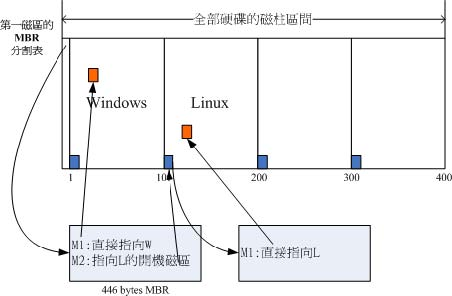
\includegraphics[width=0.55\textwidth]{boot.jpg}
	\caption{开机管理程序的工作执行示意图}
\end{figure}

在上图中我们可以发现,MBR的开机管理程序提供两个选单,选单一(M1)可以直接加载Windows的核心档案来开机; 选单二(M2)则是将开机管理工作交给第二个分区的启动扇区(boot sector)。当使用者在开机的时候选择选单事时,那举整个开机管理工作就会交给第二分区的开机管理程序了。当第二个开机管理程序启动后,该开机管理程序内(上图中)仅有一个开机选单,因此就能够使用Linux的核心档案来开机啰。 这就是多重引导的工作情况啦!我们将上图作个总结:

\begin{itemize}
	\item 每个分区都拥有自己的启动扇区(boot sector)
	\item 图中的系统槽为第一及第二分区,
	\item 实际可开机的核心档案是放置到各分区内的!
	\item loader叧会讣识自己的系统槽内的可开机核心档案,以及其他loader而已;
	\item loader可直接转向或者是间接将管理权转交给另一个管理程序。
\end{itemize}

那现在请你想一想,为什么人家常常说:『如果要安装多重引导, 最好先安装Windows再安装Linux』呢?这是因为:
\begin{itemize}
	\item Linux在安装的时候,你可以选择将开机管理程序安装在MBR或各别分区槽的启动扇区, 而且Linux的loader可以扃劢设定选单(就是上图的M1, M2...),所以你可以在Linux的boot loader里面加入Windows开机的选项;
	\item Windows在安装的时候,他的安装程序会主动的覆盖掉MBR以及自己所在分区的启动扇区,你没有选择的机会,而且他没有让我们自己选择选单的功能。
\end{itemize}

因此,如果先安装Linux再安装Windows的话,那MBR的开机管理程序就叧会有Windows的项目,而且会有Linux的项目 (因为原本在MBR内的Linux的开机管理程序就会被覆盖掉)。 那需要重新安装Linux一次吗?当然不需要,你只要用尽各种方法来处理MBR的内容即可。例如利用全中文的spfdisk(http://spfdisk.sourceforge.net/)软件来安装认识Windows/Linux的管理程序,也能够利用Linux的救援模式(secure mode)来挽救MBR即可。\footnote{详情可参考本节Windows、linux引导修复}

\subsubsection{UEFI+GPT}
由于现在win8、win10系统的用户较多,为了在使用linux的同时也能维持windows系统优秀的用户体验,我们这里讲解在最新的系统启动技术下(支持快速启动)的相关知识,以指导建立分区和安装系统。

UEFI启动是一种新的主板引导项,正被看做是有近20多年历史的BIOS的继任者。顾名思义,快速启动是可以提高开机后操作系统的启动速度。由于开机过程中UEFI的介入,使得Win 8以上的系统的开机进入系统的方式将不同于传统的开机流程。在SSD颠覆了电脑开机慢的问题之后,UEFI+Win10(也可以是其他系统)再一次颠覆我们对于开机速度的概念。

在UEFI+GPT下,计算机启动的过程就简单的多了。大概如下:计算机启动后,BIOS(EFI)将寻找第一个可启动的设备(通常为硬盘),而后从MBR(GPT)中载入启动程序,然后把控制交给这段代码。

\begin{figure}[H]
	%\usepackage{float}
	\centering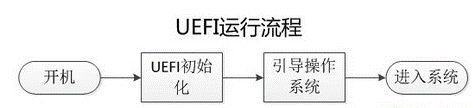
\includegraphics[width=0.8\textwidth]{uefi.png}
	\caption{UEFI运行流程}
\end{figure}

在MBR硬盘中,分区信息直接存储于主引导记录(MBR)中(主引导记录中还存储着系统的引导程序)。但在GPT硬盘中,分区表的位置信息储存在GPT头中。

\textbf{UEFI启动对比BIOS启动的优势}

\begin{enumerate}
	\item 安全性更强
	
	UEFI启动需要一个独立的分区,它将系统启动文件和操作系统本身隔离,可以更好的保护系统的启动。即使系统启动出错需要重新配置,我们只要简单对启动分区重新进行配置即可。而且,对于win8系统,它利用UEFI安全启动以及固件中存储的证书与平台固件之间创建一个信任源,可以确保在加载操作系统之前,近能够执行已签名并获得认证的“已知安全”代码和启动加载程序,可以防止用户在根路径中执行恶意代码。
	
	\item 启动配置更灵活
	
	EFI启动和GRUB启动类似,在启动的时候可以调用EFIShell,在此可以加载指定硬件驱动,选择启动文件。比如默认启动失败,在EFIShell加载U盘上的启动文件继续启动系统。
	
	\item 支持容量更大
	
	传统的BIOS启动由于MBR的限制,默认是无法引导超过2.1TB以上的硬盘的。随着硬盘价格的不断走低,2.1TB以上的硬盘会逐渐普及,因此UEFI启动也是今后主流的启动方式。
\end{enumerate}

\subsection{分区的相关知识}

\subsection{多系统的安装}

\subsubsection{U盘启动盘的制作}

获取一个启动盘是安装的第一步,一般我们为了方便快捷我们选择使用U盘做启动盘。Windows启动盘随处可见,制作简单,我们不再赘述,我们这里简要讲解一下如何使用Universal-USB-Installer制作Ubuntu启动盘。

\textbf{Universal-USB-Installer}是一个非常好用的制作Linux启动盘的工具,体积小,质量高,操作简单。\footnote{下载地址:}

除此之外,我们还要准备正版的Ubuntu镜像,一般我们从官网下载或者从可信任的镜像站下载。\footnote{下载地址:}
\begin{enumerate}

	\item 首先将U盘中有价值的文档备份,因为烧录U盘启动盘的过程可能会将U盘格式化,导致文件丢失。
	
	\item 插入U盘后运行烧录软件Universal-USB-Installer。
	
	\item 点击同意之后点开下拉菜单,选择Ubuntu。
	
	\item 之后点击Browse(浏览),找到存放Ubuntu14.04镜像的地址,确认后选择所要安装的U盘,并调节预留存储变动的空间。\footnote{注意:Set a Persistent file size for storing changes 是选择一个固定的文件存储空间,即如果你登入系统后,对系统有任何更改,将保存到U盘中,如果选择0,则不会保存。有优点也有缺点。具体可见官网给予的解释。http://www.pendrivelinux.com/what-is-persistent-linux/}

	\item 点击create之后,点击是即可进行烧录。
\end{enumerate}

至此,已经完成了Ubuntu系统启动盘的制作,非常容易。

如果你需要制作一张盘上同时可以引导多个操作系统的安装程序,你可以参考如下教程(地址:)

\subsubsection{win8(EFI)与Ubuntu14.04双系统的安装}
刘博

win8在efi引导下ubuntu的安装(b2)
(1)	在EFI(BIOS)中关闭secure boot(安全模式),目的是为了能在机器中安装非windows系统。

(2)在windows下分出30~50G的分区(具体视个人需要和机器的物理内存而定,一般交换空间大小与物理内存大小相同),下面为详细步骤:
右键我的电脑“管理”
点击磁盘管理
选择一个剩余空间较多的分区,如我的D盘,右击,压缩卷,压缩出40~50G的空间,不必新建硬盘分区,即不需要分配硬盘驱动器号。

(3)从Ubuntu官方网站上下载64位Ubuntu14.04的镜像,之后将制作好的优盘启动盘插入电脑,重新启动后更改启动选项,选择从usb HDD(usb硬盘)启动。选择“try but notinstall” 
(4)进入后可能会黑屏,这时候不要紧张,点击键盘上的亮度增加键,一般键盘上会有亮度增加标识,直接按亮度增加键或者按 Fn+亮度增加键,之后屏幕会逐渐亮起来。(这是安装有Nvida显卡的win8系统的通病)
(5)注意此时要选择其他选项: 
(6)再在Ubuntu安装过程中设置文件系统种类及其大小(新分区只能从空闲分区中往外分,如我们刚刚从D盘中分出的30~50G的空间):

<1>先分出200M 给“\\boot”设置为“主分区” ,文件系统为“ext4” 
<2>再分出20G给“\\” 设置为 “逻辑分区”(win8设置成主分区也可,因为UEFI支持超过4个主分区) ,文件系统为“ext4”  
<3>再分 10G (看用户需要)给“\\home”,设置为逻辑分区(win8设置成主分区也可,因为UEFI支持超过4个主分区),此分区在 Ubuntu系统所在分区 损坏时,其中的数据,仍可以保留。
<4>在分出 相当于物理内存大小的空间给“swap”,作为交换空间。
<5>注意要将启动器的位置安装在“\\boot”所在分区 

(7)此时重启后出现引导菜单无法引导进入win8,只能够引导进入Ubuntu,不要着急,此属正常现象,只需在BIOS中打开“secure boot”或者刚刚启动时按Fx键(选择启动项的快捷键),选择从“操作管理员”或者从“windows8”启动,或者从<EFI>/<boot>/<Microsoft>/<windows8.EFI>这条路径启动。进入win8后,用easybcd2.2(一个软件) 修复启动项(一定要提前备份启动项)。
(8)重新启动,在BIOS中关闭“secure boot”,打开快速启动,保存并重新启动。
(9)此时重新启动默认进入win8。刚开机时开机按Fx键(选择启动项的快捷键),选择 从Ubuntu启动,即可进入Ubuntu。
至此,win8 efi引导下ubuntu的安装 结束,双系统安装完毕。

\subsubsection{Q\&A}
\begin{enumerate}
	\item 进入Ubuntu安装界面的时候出现黑屏现象
	
	原因:安装有Nvida显卡的win8的通病
	
	解决方法:点击键盘上面的亮度增加键,即可点亮屏幕
	\item 安装完成系统后,无法进入Ubuntu系统,只能进入windows系统
	
	原因:默认启动时无法自动引导至Ubuntu系统
	
	解决方法:开机时通过更改启动项,更改所启动的系统
	\item 进入Ubuntu系统之后无法挂载windows系统下的硬盘
	
	原因:由于win8、win10有快速启动功能,在关机时,即会将硬盘分区锁定,所以关机后,启动至Ubuntu系统时不能挂载windows的硬盘分区,若windows重新启动,则不会对硬盘分区进行锁定
	
	解决方法:先开机至windows,之后重新启动,选择启动项启动到Ubuntu系统,此时即可访问windows的NTFS格式的硬盘分区,即可实现对硬盘的共用
\end{enumerate}

\subsubsection{WINDOWS引导修复}


1.将制作好的老毛桃u盘启动盘插入电脑中,打开电脑,在看到开机启动画面时按下相应的快捷键进入,在出现的页面中选择u盘启动即可进入到老毛桃u盘启动盘主界面,然后使用上下方向键将光标移动至“【02】运行老毛桃Win2003PE增强版(装机推荐)”按下回车键;如下图所示:

2.当进入到winpe系统后双击pe桌面上的“windows启动引导修复”工具,在弹出的窗口中点击“开始修复”,如下图所示:

3.接着系统就会自动的进行系统引导修复,当修复完成后会建立一个报告;如下图所示:

4.通过修复后的报告我们可以查看到修复后的结果;如下图所示:

接下来只要进行重启系统即可正常进入windows系统桌面了。

\subsubsection{Linux引导修复}

GRUB是一个来自GNU的多操作系统启动程序。GRUB是多启动规范的实现,他允许用户可以在计算机内同时拥有多个操作系统,并在计算机启动时选择希望运行的操作系统。GRUB可用于选择操作系统分区上的不同内核,也可用于向这些内核传递启动参数。在UBUNTU中,默认的存储位置是/BOOT/GRUB,因为我们只是单纯的进行修改与学习,所以我们利用例如GEDIT进行对GRUB.CFG的修改具体命令行参数为进行操作之后可以对GRUB.CFG进行修改。

\begin{enumerate}
	\item 调整默认启动顺序
	在系统启动GRUB进行选择界面时会有这样的界面默认第一个的INDEX为0之后要记住你希望调整的位置之后在GRUB.CFG找到如下代码
	将 SET DEFAULT="0"改为调整位置的INDEX编码
	\item 修复GRUB的步骤
	\subitem 想办法进入到UBUNTU的LIVE CD系统,或者其他较新版本的LIVE CD系统。
	\subitem 打开终端,输入SUDO FDISK -L,查看ID=83的分区,记录下SD[NUM],比如SDA8。
	\subitem 如果上一步中存在多个ID=83的分区,自己想办法确定/分区所在的分区号,并且/BOOT也是和/分区挂载在同一个分区上,比如就是SDA8。
	\subitem 输入SUDO -I,获得ROOT权限。
	\subitem MKDIR /MEDIA/TMP。
	\subitem 将/分区挂载到新建的目录MOUNT /DEV/SDA8 /MEDIA/TMP。
	\subitem 如果以前的系统/BOOT是单独挂载的话,则需要找到/BOOT的分区如SDA7,然后MOUNT /DEV/SDA7 /MEDIA/TMP/BOOT。否则这一步直接跳过去。
	\subitem 接下来准备安装GRUB了,终端输入:GRUB-INSTALL --ROOT-DIRECTORY=/MEDIA/TMP /DEV/SDA。
	\subitem 如果看到INSTALLATION FINISHED, NO ERROR OCCURED之类的信息时表明已经成功了。
	\subitem 此时重启系统,应该可以看到原来的GRUB2引导界面回来了,并且如果有其他系统存在的话,也会显示启动项列表中
\end{enumerate}




\section{Ubuntu的使用}
在Ubuntu上安装开源软件较windows要方便的多,其中最主要的原因就是有了一些安装
\subsection{软件安装之软件源(apt-get)}
 给苹果手机越过狱的同学可能对软件源这个名字不太陌生。软件源是Linux系统的应用程序安装仓库,很多应用软件都会这收录到这个仓库里面。软件源可以是网络服务器,是光盘,甚至是硬盘上的一个目录。
 
 使用软件源安装软件很方便,只需要一条命令.(sudo apt-get install <软件包名> )。
 用软件源安装的软件跟随系统更新,省去很多操作。
 软件源安装的软件都有数字签名,能有效防止恶意软件。
   

  软件源都放在路径为/etc/apt下的sources.list文件内,用文本编辑器打开文件就可以对计算机内的软件源进行添加与删除。
  在终端输入sudo gedit /etc/apt/sources.list,文本编辑器打开的 sources.list就是添加源的文件,只要把找到的源地址添加到文件最后一行,然后在终端运行sudo apt-get update更新配置.
  
   配置文件的格式:
   [软件源地址][发行版地址][包类型]
   
   配置文件类型:
   \begin{itemize}
   	\item main: Canonical公司支持的免费和开源软件
   	\item universe:社区维护的免费和开源软件
   	\item restricted:设备的专有驱动
   	\item multiverse:有版权和合法性问题的软件
   \end{itemize}
   
  我们建议使用中科大或是阿里云的源服务器\footnote{这里放网址,表明版权引用},这两个源更新速度快、软件包全,不过在使用的时候一定要注意对应的Ubuntu版本号,否则会产生一些意想不到的错误。
   
 之前讲过Apt安装软件非常方便,只需要一个命令便可以自动处理依赖关系并安装软件,软件的安装卸载命令如下
 \begin{Code}
 •sudo apt-get install  <软件名> 安装某软件
 •sudo apt-get install  <软件名> --reinstall 重新安装某软件
 •sudo apt-get remove <软件名> 卸载软件
 •sudo apt-get purge <软件名>  卸载某软件,并且清理软件遗留配置文件
 •apt-cache search <字符串> 搜索名称含有字符串的软件
 \end{Code}
 
 apt还有一些其他的命令用来管理软件源和软件包,其中涉及源更新、软件升级、清理软件包等等。
  \begin{Code}
 •sudo apt-get update 更新软件包列表
 •sudo apt-get upgrade 对已安装的软件进行更新
 •sudo apt-get dist-upgrade 对发行版进行升级,可能有新软件包的升级与旧软件包的删除(ubuntu) 发行版升级(debian)
 •sudo do-release-upgrade 手动发行版升级ubuntu
 •sudo apt-get autoremove 移除无用软件包(非手动安装而不被依赖)
 •sudo apt-get autoclean 清理无用的本地安装包缓存
 •sudo apt-get clean 清理所有的本地安装包缓存,缓存路径(/var/cache/apt/archives)
  \end{Code}

 推荐一些图形工具,对于刚接触ubuntu的人可以使用这些工具方便软件的安装和管理。
 
 ubuntu 软件中心:类似于手机的应用商店,一键安装,部分软件付费。
 
 \textbf{新立得软件包管理器}:类似于android的应用商店,可以直接获取软件,一键安装,并且便于软件的更新。
\subsection{软件安装之编译安装}
 当然不是所有的软件都在源上都有,比如在一些开源社区上的工具,往往为了适配更多的平台,都没有直接制作安装包,这时候就要我们自己编译然后再安装到我们的电脑上。这种安装方法虽然有些复杂但也是必要的,
 
\subsubsection{什么是编译安装}
 编译安装简单来说就是根据源码编译出软件(把源码编译成可执行二进制代码),然后对软件进行安装.
 在编译安装之前需要安装编译所需软件包,如gcc,g++,automake,build-essential等.得到的源代码包文件通常为XXX.tar.gz ,XXX.tar.xz,XXX.tar.bz2等格式,实际上是一个压缩文件.
\subsubsection{编译安装流程}
\begin{enumerate}
	\item  tar xvf xxx.tar.gz 解压源码包  
	\item 在终端中进入解压文件目录,并在编译前阅读解压文件中的README和INSTALL文件确定安装方式和所需依赖.
	\item  ./configure  配置编译参数,最常见的是prefix=安装路径,如果不改变则默认把软件安装到系统的文件结构中.
	\item  make 当上一步正确的执行后会生成一个Makefile文件,使用make命令可以对软件源码进行编译
	\item  make install 安装(可能会需要root权限)
\end{enumerate}
 部分软件还会提供make test 这样的测试,在安装前可以运行make test 来测试软件是否编译正确。

\section{shell的使用}
Shell,在计算机科学中又称壳(相对于核来说)。操作系统与外部最主要的接口就叫做shell。
shell管理你与操作系统之间的交互:等待你输入,向操作系统解释你的输入,并且处理各种各样的操作系统的输出结果。shell提供了你与操作系统之间通讯的方式。简单的可以理解成一种可以编译的,可执行的一种语言。
\subsection{常见的shell}
在Linux中,由于命令行的高效率,shell是主要的工作阵地。如今的shell的使用场所已经主要以模拟终端的形式出现在操作系统中,比如windows里的cmd和powershell,Ubuntu里的terminal。上面讲了shell是一种语言,在shell的发展过程中也产生好多个版本,主要有下面这些:
\begin{itemize}
	\item sh :是Steve Bourne在AT\&T贝尔实验室创造的Bourne shell的简称
	\item Bash: 在GUN计划的赞助下免费软件基金会的Brian Fox开发了bash, 是Bourne again shell的简称
	\item Ksh:Ksh shell由AT\&T贝尔实验室的David Korn开发,是sh shell的前身。它是UNIX System V系统中默认和最常用的shell。
	\item Csh: Bill Joy开发了csh shell,并被多数Berkeley UNIX系统(例如Sun Microsystems的产品)作为默认shell。
	\item Tcsh:Tcsh shell是C shell(csh)的开放源代码版本。
	\item Ash:Ash shell是Berkeley UNIX sh shell的简化版本。Kenneth Almquist开发了ash shell。 
	\item Ash shell是可以在系统资源较少的嵌入式系统中使用的一种很好的shell.
	\item Zsh:Zsh 是shell的另一个克隆,提供了很多人性化的设计,非常好用,推荐。
\end{itemize}


shell作为一个脚本语言,主要的元素还是由命令组成,shell命令的使用方法非常简单,从这里我们开始学习shell。

\subsection{Shell命令}

Linux是一个多用户多任务的操作系统,也是一款自由软件,完全兼容POSIX标准,拥有良好的用户界面,支持多种处理器架构,移植方便。Linux 中有大量常用的命令,可以方便我们快速进行操作,值得花时间去掌握。

\subsubsection{命令帮助} 

在linux终端,面对命令不知道怎么用,或不记得命令的拼写及参数时,我们需要求助于系统的帮助文档; linux系统内置的帮助文档很详细,通常能解决我们的问题,我们需要掌握如何正确的去使用它们。
\begin{itemize}
\item 在只记得部分命令关键字的场合,我们可通过man -k来搜索;
\item 需要知道某个命令的简要说明,可以使用whatis;而更详细的介绍,则可用info命令;
\item 查看命令在哪个位置,我们需要使用which;
\item 而对于命令的具体参数及使用方法,我们需要用到强大的man;
\end{itemize}


简要说明命令的作用(显示命令所处的man分类页面):

\begin{Code}
$ whatis command
$ whatis -w "loca*"  //正则匹配:
$ info command       //更加详细的说明文档
\end{Code}

查询命令command的说明文档:

\begin{Code}
$ man command
eg:man date
\end{Code}

在man的帮助手册中,将帮助文档分为了9个类别,对于有的关键字可能存在多个类别中, 我们就需要指定特定的类别来查看;(一般我们查询bash命令,归类在1类中);man页面所属的分类标识(常用的是分类1和分类3)
\begin{enumerate}
\item 用户可以操作的命令或者是可执行文件
\item 系统核心可调用的函数与工具等
\item 一些常用的函数与数据库
\item 设备文件的说明
\item 设置文件或者某些文件的格式
\item 游戏
\item 惯例与协议等。例如Linux标准文件系统、网络协议、ASCⅡ,码等说明内容
\item 系统管理员可用的管理条令
\item 与内核有关的文件
\end{enumerate}


前面说到使用whatis会显示命令所在的具体的文档类别,如下:


\begin{Code}
$ whatis printf
printf               (1)  - format and print data
printf               (1p)  - write formatted output
printf               (3)  - formatted output conversion
printf               (3p)  - print formatted output
printf [builtins]    (1)  - bash built-in commands, see bash(1)
\end{Code}

我们看到printf在分类1和分类3中都有;分类1中的页面是命令操作及可执行文件的帮助;而3是常用函数库说明;如果我们想看的是C语言中printf的用法,可以指定查看分类3的帮助:

\begin{Code}
$ man 3 printf
\end{Code}

\subsubsection{文件、目录管理}  

\textbf{文件创建和删除}

\begin{itemize}
\item 创建:mkdir
\item 删除:rm
\item 删除非空目录:rm -rf file
\item 删除日志 \textbf{rm *log}
\item 移动:mv
\item 复制:cp (复制目录:cp -r )
\end{itemize}

\textbf{目录切换,打印}

\begin{itemize}
	\item 找到文件/目录位置:cd path
	\item 显示当前路径: pwd
	\item 显示当前目录下的文件:ls
	\item 按时间排序,以列表的方式显示目录项:ls -lrt
\end{itemize}

\textbf{查看当前目录下文件个数}

\begin{Code}
    $ find ./ | wc -l
\end{Code}


\textbf{查找文件或目录}
\begin{Code}
    $ find ./ -name '*.o'  //递归查找当前目录及子目录所有的.o文件
\end{Code}

find是实时查找,如果需要更快的查询,可试试locate;locate会为文件系统建立索引数据库,如果有文件更新,需要定期执行更新命令来更新索引库:

\begin{Code}
    $ locate string     //寻找包含有string的路径,
    $ updatedb
\end{Code}    

与find不同,locate并不是实时查找。你需要更新数据库,以获得最新的文件索引信息。

\textbf{查看文件}:cat vi head tail more

\begin{Code}
$ cat -n                // 显示时同时显示行号
$ head -10 filename     // 只看前10行:
$ tail -5 filename      // 显示文件倒数五行
$ diff file1 file2      // 查看两个文件间的差别
\end{Code}

\textbf{文件与目录权限修改}

\begin{itemize}
\item 改变文件的拥有者:chown
\item 改变文件读、写、执行等属性:chmod
\item 递归子目录修改:chown -R user source/
\item 增加脚本可执行权限:chmod +x filename
\end{itemize}


\textbf{创建符号链接/硬链接}

\begin{itemize}
\item ln sourcefile destfile:硬连接;删除一个,将仍能找到;
\item ln -s sourcefile destfile:符号链接(软链接);删除源,另一个无法使用;
\end{itemize}

\subsubsection{进程、作业管理} 

\textbf{ps命令}用于报告当前系统的进程状态。可以搭配kill指令随时中断、删除不必要的程序。ps命令是最基本同时也是非常强大的进程查看命令,使用该命令可以确定有哪些进程正在运行和运行的状态、进程是否结束、进程有没有僵死、哪些进程占用了过多的资源等等,总之大部分信息都是可以通过执行该命令得到的。 

    ps (选项)

选项有很多,常用的如下:
\begin{itemize}
\item a:显示现行终端机下的所有程序,包括其他用户的程序。
\item u:以用户为主的格式来显示程序状况。
\item x:显示所有程序,不以终端机来区分。 
\end{itemize}

\textbf{top命令}可以实时动态地查看系统的整体运行情况,是一个综合了多方信息监测系统性能和运行信息的实用工具。通过top命令所提供的互动式界面,用热键可以管理。

运行 top 命令后,CPU 使用状态会以全屏的方式显示,并且会处在对话的模式,此时用基于 top 的命令,可以控制显示方式。对于进程,平时我们最常想知道的就是哪些进程占用CPU最多,占用内存最多。以下两个命令就可以满足要求:
\begin{itemize}
\item P:根据CPU使用百分比大小进行排序。
\item M:根据驻留内存大小进行排序。
\item i:使top不显示任何闲置或者僵死进程。
\end{itemize}

\textbf{kill命令}用来删除执行中的程序或工作。kill可将指定的信息送至程序。预设的信息为SIGTERM(15),可将指定程序终止。若仍无法终止该程序,可使用SIGKILL(9)信息尝试强制删除程序。程序或工作的编号可利用ps指令或job指令查看。 

一般情况下,我们先用 ps 查找指定进程,然后用 kill 杀掉,如下:

\begin{Code}
ps -ef | grep vim 
root 3268 2884 0 16:21 pts/1 00:00:00 vim install.log 
root 3370 2822 0 16:21 pts/0 00:00:00 grep vim 

kill 3268 
kill 3268
-bash: kill: (3268) - 没有那个进程 
\end{Code}

\textbf{ipcs命令}用于报告Linux中进程间通信设施的状态,显示的信息包括消息列表、共享内存和信号量的信息。 
\begin{itemize}
\item -a:显示全部可显示的信息;
\item -q:显示活动的消息队列信息; 
\item -m:显示活动的共享内存信息; 
\item -s:显示活动的信号量信息。
\end{itemize}

例如:
\begin{Code}
ipcs -a 
------ Shared Memory Segments -------- 
key        shmid   owner perms bytes   nattch status 
0x7401833d 2654208 root  600   4 0 
0x00000000 3145729 root  600   4194304 9      dest 
0x7401833c 2621442 root  600   4       0 
0xd201012b 3080195 root  600   1720    2 
\end{Code}

\textbf{ipcrm命令}用来删除一个或更多的消息队列、信号量集或者共享内存标识。

在linux环境下,任何事物都以文件的形式存在,通过文件不仅仅可以访问常规数据,还可以访问网络连接和硬件。所以如传输控制协议 (TCP) 和用户数据报协议 (UDP) 套接字等,系统在后台都为该应用程序分配了一个文件描述符,无论这个文件的本质如何,该文件描述符为应用程序与基础操作系统之间的交互提供了通用接口。

因为应用程序打开文件的描述符列表提供了大量关于这个应用程序本身的信息,因此通过\textbf{lsof命令}能够查看这个列表对系统监测以及排错将是很有帮助的。 主要有下面这些选项:
\begin{itemize}
\item -a:列出打开文件存在的进程; 
\item -c<进程名>:列出指定进程所打开的文件; 
\item -d<文件号>:列出占用该文件号的进程; 
\item +d<目录>:列出目录下被打开的文件; 
\item -i<条件>:列出符合条件的进程。(4、6、协议、:端口、 @ip ) 
\item -p<进程号>:列出指定进程号所打开的文件;
\end{itemize}
\textbf{jobs命令} 用于显示Linux中的任务列表及任务状态,包括后台运行的任务。该命令可以显示任务号及其对应的进程号。其中,任务号是以普通用户的角度进行的,而进程号则是从系统管理员的角度来看的。一个任务可以对应于一个或者多个进程号。 

其中,输出信息的第一列表示任务编号,第二列表示任务所对应的进程号,第三列表示任务的运行状态,第四列表示启动任务的命令。 

在Linux系统中执行某些操作时候,有时需要将当前任务暂停调至后台,或有时须将后台暂停的任务重启开启并调至前台,这一序列的操作将会使用到 jobs、bg、和 fg 三个命令以及两个快捷键来完成。\textbf{ctrl + z} 可以将一个正在前台执行的命令放到后台,并且暂停。

\begin{Code}
fg %jobnumber  # 将后台中的命令调至前台继续运行
               #(%jobnumber是通过jobs命令查到的后台正在执行的命令的序号(不是pid))
bg %jobnumber  # 将一个在后台暂停的命令,变成继续执行。
\end{Code}

\subsubsection{网络命令} 

\textbf{ifconfig命令}被用于配置和显示Linux内核中网络接口的网络参数。用ifconfig命令配置的网卡信息,在网卡重启后机器重启后,配置就不存在。要想将上述的配置信息永远的存的电脑里,那就要修改网卡的配置文件了。

\textbf{iptables命令}是Linux上常用的防火墙软件,是netfilter项目的一部分。可以直接配置,也可以通过许多前端和图形界面配置。 

\textbf{route命令}用来显示并设置Linux内核中的网络路由表,route命令设置的路由主要是静态路由。直接在命令行下执行route命令来添加路由,不会永久保存,当网卡重启或者机器重启之后,该路由就失效了;可以在/etc/rc.local中添加route命令来保证该路由设置永久有效。

\textbf{netstat命令}用来打印Linux中网络系统的状态信息,可让你得知整个Linux系统的网络情况。可以显示相关的网络信息,如接口/网卡状态(-i),路由表(-r),网络连接(-a),tcp相关选项(-t),udp相关选项(-u),按各个协议统计(-s)。例如:

\begin{Code}
netstat -a #列出所有端口 
netstat -at #列出所有tcp端口 
netstat -au #列出所有udp端口 
netstat -l #只显示监听端口 
netstat -lt #只列出所有监听 tcp 端口 
netstat -lu #只列出所有监听 udp 端口 
netstat -lx #只列出所有监听 UNIX 端口
\end{Code}

\textbf{tcpdump命令}是一款sniffer工具,它可以打印所有经过网络接口的数据包的头信息,也可以使用-w选项将数据包保存到文件中,方便以后分析。如下:

\begin{Code}
tcpdump host 210.27.48.1                # 截获所有210.27.48.1 的主机收到的和发出的所有的数据包
tcpdump tcp port 23 host 210.27.48.1    # 获取主机210.27.48.1接收或发出的telnet包
tcpdump udp port 123                    # 对本机的udp 123 端口进行监视
\end{Code}

\textbf{scp命令}可以将本地localpath指向的文件上传到远程主机的path路径,或者遍历下载path路径下的整个文件系统,到本地的localpath:

\begin{Code}
$ scp localpath ID@host:path
$ scp -r ID@site:path localpath
\end{Code}

\subsubsection{其它命令} 

\textbf{free命令}可以显示当前系统未使用的和已使用的内存数目,还可以显示被内核使用的内存缓冲区。
\begin{itemize}
\item uname -a   \# 查看内核/操作系统/CPU信息
\item hostname   \# 查看计算机名
\item env        \# 查看环境变量
\item uptime     \# 查看系统运行时间、用户数、负载
\end{itemize}

\textbf{useradd命令}用于Linux中创建的新的系统用户。useradd可用来建立用户帐号。帐号建好之后,再用passwd设定帐号的密码,而可用\textbf{userdel}删除帐号。使用useradd指令所建立的帐号,实际上是保存在/etc/passwd文本文件中。

新建一个管理员用户admin,可以用下面命令:

\begin{Code}
useradd -u 0 -o admin
\end{Code}

-u 因为系统用户的用户号为0,故指定用户号为0;因为系统本身存在用户号为0的系统用户,故应该用-o选项,重复使用其他用户的标识号。



\subsubsection{更多阅读} 
[[新建管理员用户](http://www.nowcoder.com/questionTerminal/43d2ccded19445b18ec61069416c299f)]

[为什么计算机的学生要学习 Linux 开源技术](http://www.tinylab.org/why-computer-students-learn-linux-open-source-technologies/) 
   
[工具参考篇](http://linuxtools-rst.readthedocs.org/zh_CN/latest/tool/index.html)  

[Linux 命令大全](http://man.linuxde.net/)  

[学会使用命令帮助](http://linuxtools-rst.readthedocs.io/zh_CN/latest/base/01_use_man.html)  

\subsection{脚本编写}
通常我们把上面这些命令根据一定的语法,组合之后成为一个shell文件,赋予执行权限之后便可以进行自动化操作,这个文件我们称作脚本文件。下面我么通过下面几个方面简单地讲解一下如何编写脚本文件。

建立一个文件并将扩展名修改为.sh,之后用任何文本编辑器打开,键入便开始编写脚本了。

\subsubsection{一个简单的脚本}
这里我们引用《鸟哥的私房菜》的习惯。
鸟哥主要将整个程序的撰写分成数段,大致是这样:

\begin{Code}
	[root@www ~]# mkdir scripts; cd scripts 
	[root@www scripts]# vi sh01.sh 
	#!/bin/bash 
	# Program: 
	# This program shows "Hello World!" in your screen. 
	# History: 
	# 2005/08/23 VBird First release 
	PATH=/bin:/sbin:/usr/bin:/usr/sbin:/usr/
	local/bin:/usr/local/sbin:~/bin export 
	PATH 
	echo -e "Hello World! \a \n" exit 0


1. 第一行 #!/bin/bash 在宣告这个脚本使用的 shell 名称: 因为我们使用的是 bash ,所以,必须要以『 #!/bin/bash 』来宣告这个档案内的语法使用 bash 的语法!那举当这个程序被执行时,他就能够加载 bash 的相关环境配置文件 (一般来说就是 non-login shell 的 ~/.bashrc), 幵且执行 bash 来使我们底下的指令能够执行!这很重要的!(在很多状况中,如果没有设定好这一行, 那举该程序很可能会无法执行,因为系统可能无法判断该程序需要使用什么 shell 来执行啊!)

2. 程序内容的说明: 整个脚本当中,除了第一行的『 #! 』』是用来宣告 shell 的之外,其他的 # 都是『批注』用途! 所以上面的程序当中,第二行以下就是用来说明整个程序的基本数据。一般来说, 建议你一定要养成说明该脚本的:1. 内容不功能; 2. 版本信息; 3. 作者不联络方式; 4. 建档日期;5. 历史纪录 等等。这将有助于未来程序的改写与 debug 呢!

3. 主要环境变量的宣告: 建议务必要将一些重要的环境变量设定好,鸟哥个人认为, PATH 与 LANG (如果有使用到输出相关的信息时) 是当中最重要的! 如此一来,则可让我们这支程序在运行时,可以直接下达一些外部指令,而不必写绝对路径呢!比较好啦!

4. 主要程序部分 就将主要的程序写好即可!在这个例子当中,就是 echo 那一行啦!

5. 执行成果告知 (定义回传值) 
一个指令的执行成功与否,可以使用 \$? 这个发量来观察~ 那么我们也可以利用 exit 这个指令来让程序中断,并且回传一个数值给系统。 在我们这个例子当中,鸟哥使用 exit 0 ,这代表离开脚本幵且回传一个 0 给系统, 所以我执行完这个脚本后,若接着下达 echo \$? 则可得到 0 的值喔! 更聪明的读者应该也知道了,呵呵!利用这个 exit n (n 是数字) 的功能,我们还可以自定义错误讯息, 让这支程序发得更加的 smart 呢!

\end{Code}
接下来透过刚刚上头介绍的执行方法来执行看看结果吧!
\begin{Code}
	[root@www scripts]# sh sh01.sh
	Hello World !
\end{Code}
\subsubsection{好的脚本习惯}
在一些环境的设定上面,毕竟每个人的环境都不相同,为了取得较佳的执行环境, 我都会自行先定义好一些一定会被用到的环境发量,例如 PATH 这个玩意儿! 这样比较好啦~所以说,建议你一定要养成良好的脚本撰写习惯,在每个脚本的文件头处记录好:
\begin{enumerate}
	\item 脚本的功能;
	\item 脚本的版本信息;
	\item 脚本的作者与联系C方式;
	\item 脚本的版权宣告方式;
	\item 脚本的 History (历史纪录);
	\item 脚本内较特殊的指令,使用『绝对路径』的方式来下达;
	\item 脚本运作时需要的环境发量预先宣告与设定。
\end{enumerate}

除了记录这些信息之外,在较为特殊的程序代码部分,个人建议务必要加上批注说明,可以帮助你非常非常多! 此外,程序代码的撰写最好使用巢状方式,在包覆的内部程序代码最好能以 [tab] 按键的空格向后推, 这样你的程序代码会显的非常的漂亮与有条理!在查阅不 debug 上较为轻松愉快喔! 另外,使用撰写脚本的工具最好使用 vim 而不是 vi ,因为 vim 会有额外的语法检验机制,能够在第一阶段撰写时就发现语法方面的问题喔!

\subsubsection{流程控制}

流程控制是任何编程语言中很常用的部分,在bash中也使用if/else,while,until,for等语句来控制流程。
常见的流程控制用法如下:

用if/else控制:
\begin{Code}
if cmda; then
cmd1;
elif cmdb; then
cmd2;
else cmdc; then
cmd3; 
fi
\end{Code}
用while或until控制:
\begin{Code}
while cmd1; do
cmd2;
done
\end{Code}
for条件语句控制:
\begin{Code}
for name in words; do
cmd;
done

for ( (exp1;exp2;exp3));do
cmd;
done
\end{Code}
case条件语句控制:
\begin{Code}
case word in
part1) cmd1;;
part2) cmd2;;
part3) cmd3;;
esac

\end{Code}

举例:for控制语句与数组

\begin{Code}
a=”1 2 3 4 5 a b c”

for I in $a; do
echo $i
done


a=(1 2 3 4 5 a b c)
for ( (i=0;i<10;++i) );do
echo $i
echo ${a[i]}
done
\end{Code}

在这个例子中,有\$符号,\$与其它字符魔术变量,魔术变量对应着特定的语义,如下:

\begin{Code}
$#		argc
$0		argv[0]
$1		argv[1]
${11}	argv[11]
$?		上一句的返回值
$$  		当前bash进程的PID
$-		当前bash的参数
$*		作为一个整体的参数
$@		分词后的参数
\end{Code}


\subsubsection{输入输出}

在 Bash 命令执行的过程中,主要有三种输出入的状况,分别是:

\begin{Code}
	1. 标准输入;代码为 0 ;或称为 stdin ;使用的方式为 <
	2. 标准输出:代码为 1 ;或称为 stdout;使用的方式为 1>
	3. 错误输出:代码为 2 ;或称为 stderr;使用的方式为 2>
\end{Code}

在shell里我们使用”>”和”<”两个符号来重定向输入与输出流,比如:

\begin{Code}	
	ls > file_list		输出到一个文件,覆盖原来的文件
	ls >> file_list       输出重定向到一个文件,追加原来的文件
\end{Code}

重定向符号与标准错误重定向规则如下:

\begin{Code}
	重定向符号:
	>	输出重定向到一个文件或设备 覆盖原来的文件
	>!	输出重定向到一个文件或设备 强制覆盖原来的文件
	>>	输出重定向到一个文件或设备 追加原来的文件
	<	反向输出输入重定向
	标准错误重定向符号:
	2>	将一个标准错误输出重定向到一个文件或设备 覆盖原来的文件
	2>>	将一个标准错误输出重定向到一个文件或设备 追加到原来的文件
	2>&1将一个标准错误输出重定向到标准输出
	>&	将一个标准错误输出重定向到一个文件或设备 覆盖原来的文件
	|&	将一个标准错误 管道 输送 到另一个命令作为输入
\end{Code}
在最后一条规则里面提到了管道这个名词,管道的符号为“|”,其作用是拼接多个程序的输入与输出,即将前一个程序的输出输入到下一个程序作为下一个程序的输入。

假设我们想要知道 /etc/ 底下有多少档案,那么可以利用 ls /etc 来查阅,不过,因为 /etc 底下的档案太多,导致一口气就将屏幕塞满了,从而不知道前面输出的内容是啥。此时,我们可以透过 less 指令的协助,利用:
\begin{Code}
	[root@linux ~]# ls -al /etc | less
\end{Code}
如此一来,使用 ls 指令输出后的内容,就能够被 less 读取, 并且利用 less 的功能,我们就能够前后翻动相关的信息了!

注意:这个管线命令“|” 仅能处理经由前面一个指令传来的正确信息,也就是 standard output( stdout ) 的信息,对于 stdandard error 并没有直接处理的能力,请记得。

创建文件:
\begin{Code}
	touch newfile
	> newfile
	
	echo “something” > file
\end{Code}
\subsubsection{脚本编写实践}
\begin{Code}
#!/bin/bash
#=======================================================
# Agent2D-3.1.0 start script
# RoboCup2D @ Anhui Unversity of Technology
# Bugs or Suggestions please mail to guofeng1208@163.com
#=======================================================


if [ -z "$LD_LIBRARY_PATH" ]
then
LD_LIBRARY_PATH=.
else
LD_LIBRARY_PATH=.:$LD_LIBRARY_PATH
fi

export LD_LIBRARY_PATH


host="localhost"
port=6000
coach_port=6002
teamname="YuShan2015"

player="./YuShan2015_Player"
coach="./YuShan2015_Coach"

config="./data/player.conf"
coach_config="./data/coach.conf"
config_dir="./data/formations-dt"

opt="--player-config ${config} --config_dir ${config_dir}"
coachopt="--coach-config ${coach_config} --use_team_graphic on"


sleeptime=0.5
posnum=0
count=12


usage()
#usage函数
#显示下面的内容直至EOF
{
	cat << EOF
	
	Usage: $0  [options]

	Options:
	-help               Show help infomation
	-h      (IP)        Special server host address
	-p      (port)      Special the server port number of player
	-t      (Name)      Special teamname
	-c      (number)    Special player amount(start with 1)
	-n      (number)    Special player position number(Not uniform)
	EOF
}


if [ $# -eq 1 -a "$1" = "-help" ]
#如果参数数量=1且$1=-help执行usage(-a表示两个条件同时成立)
then
usage
exit 0
fi


while getopts "h:p:t:c:n:" flag
#当输入上的字符是h p t c n中的一个时将其值赋予flag
do
case "$flag" in
h)
host=$OPTARG
;;
p)
port=$OPTARG
coach_port=$((port+2))
;;
t)
teamname=$OPTARG
;;
c)
count=$OPTARG
;;
n)
posnum=$OPTARG
;;
*)
echo "Error cmdline option"
usage
exit 1
esac
done
#当$flag为h时令当前值赋予host


opt="${opt} -h ${host} -p ${port} -t ${teamname}"
coachopt="${coachopt} -h ${host} -p ${coach_port} -t ${teamname}"
#已经定义的参数搭配


# the limit of core dump file size 
ulimit -f unlimited


if [ $posnum -ne 0 ]
#参数$posnum是否不等于0
then
case $posnum in
1)
${player} ${opt} -g -n $posnum &
;;
12)
${coach} ${coachopt}  &
;;
*)
${player} ${opt} -n $posnum  &
;;
esac

exit 0
fi
#当$posnum为1时执行${player} ${opt} -g -n $posnum,即球员的部分
#当$posnum为12时执行${coach} ${coachopt},即教练的部分
#其余的部分执行${player} ${opt} -n $posnum,即球员的部分

i=1

while [ ${i} -le ${count} ]
#${i}小于等于${count}时
do
case ${i} in
1)
echo "team $teamname: Start Player $i"
${player} ${opt} -g &
;;
12)
echo "team $teamname: Start Coach"
${coach} ${coachopt} &
;;
*)
echo "team $teamname: Start Player $i"
${player} ${opt} &
;;
esac

sleep $sleeptime
i=$((i+1))
done
#利用while中的i=$((i+1))使11个球员和一个教练都能参与
#当${i}为1时显示“team $teamname: Start Player $i”执行 ${player} ${opt} -g,即球员的部分
#当${i}为12时时显示"team $teamname: Start Coach"执行 ${coach} ${coachopt},即教练的部分
#当${i}为其它值时输出"team $teamname: Start Player $i"执行 ${player} ${opt}
#$为后台执行
exit 0
\end{Code}


\chapter{C++编程基础}

由于这只是一个有关机器人足球的技术文档,不在这里赘述过多C++知识,
仅在此提供一个由c语言基础过度到C++的简易教程。更多的知识请参照
C++ primer plus。\footnote{<<C++ primer plus (第6版)>> }
\section{c++对c的扩充}
\subsection{文件名称}
在C语言中,源文件的拓展名为”.c”,头文件的拓展名为”.h”,在C++语言中源文件的拓展名由“.c”变更为了”.cpp”,而头文件依然可以使用C语言中的拓展名”.h”

在使用include对文件进行包含时,C语言需要加上文件”.h”拓展名而C++则可以仅使用文件名。

C语言文件包含

\begin{Code}
#include<iostream.h>
\end{Code}

C++文件包含
\begin{Code}
#include<iostream>
\end{Code}

由于C++为C语言发展而来,C++保留了一部分C的规定,使得C++可以很好的兼容C语言,所以在C++中以下文件的包含方式也是可以的。

C++文件包含
\begin{Code}
#include<iosteam.h>
\end{Code}
\subsection{命名空间}
命名空间为面向对象程序设计的重要概念之一,他可以通过将用户定义的函数或类放置在一个命名空间中的方法来防止用户定义的函数或类与他人的定义发生重名。

命名空间的定义:

\begin{Code}
namespace 名称
{
	内容
}
\end{Code}

命名空间的访问:

\begin{Code}
名称::内容
\end{Code}

命名空间的使用:

\begin{Code}
using namespace 名称;
\end{Code}

\subsection{标准输入输出}
C++在进行输入及输出时除了可以使用C语言中的prinyf与scanf函数外,还可以使用C++中提供的cin和cout流对象。

\subsubsection{使用cout进行输出}
在使用cout进行输出时需要在被输出项前加<<符号,需要注意的是每一个输出项使用一个<<符号而不可以多个输出项共用一个。并且如果在输出时没有指定输出的数据类型的话,系统会以输出项被定义的类型进行输出。


\begin{Code}
int a = 1;
float b = 3.5;
char c = ‘x’

正确输出方式 cout << a << b << c;
错误输出方式 cout << a,b,c;
输出结果:13.5x
\end{Code}

\subsubsection{使用cin进行输入}



\subsection{动态内存分配与释放}
C/C++定义了4个内存区间:
代码区,全局变量与静态变量区,局部变量区即栈区,动态存储区,即堆(heap)区或自由存储区(free store)。

\subsubsection{堆的概念}
通常定义变量(或对象),编译器在编译时都可以根据该变量(或对象)的类型知道所需内存空间的大小,从而系统在适当的时候为他们分配确定的存储空间。这种内存分配称为静态存储分配;
有些操作对象只在程序运行时才能确定,这样编译时就无法为他们预定存储空间,只能在程序运行时,系统根据运行时的要求进行内存分配,这种方法称为动态存储分配。所有动态存储分配都在堆区中进行。

当程序运行到需要一个动态分配的变量或对象时,必须向系统申请取得堆中的一块所需大小的存贮空间,用于存贮该变量或对象。当不再使用该变量或对象时,也就是它的生命结束时,要显式释放它所占用的存贮空间,这样系统就能对该堆空间进行再次分配,做到重复使用有限的资源。
\subsubsection{堆内存的分配与释放}
\textbf{堆空间申请、释放的方法:}

在C++中,申请和释放堆中分配的存贮空间,分别使用new和delete的两个运算符来完成:

\begin{Code}
指针变量名=new 类型名(初始化式);
delete 指针名;
\end{Code}
例如:
\begin{Code}
int *pi=new int(0);
\end{Code}

它与下列代码序列大体等价:
\begin{Code}
int ival=0, *pi=&ival;
\end{Code}
区别:pi所指向的变量是由库操作符new()分配的,位于程序的堆区中,并且该对象未命名。  

\textbf{堆空间申请、释放说明:}

\begin{enumerate}
	\item new运算符返回的是一个指向所分配类型变量(对象)的指针。对所创建的变量或对象,都是通过该指针来间接操作的,而且动态创建的对象本身没有名字。
	\item 一般定义变量和对象时要用标识符命名,称命名对象,而动态的称无名对象(请注意与栈区中的临时对象的区别,两者完全不同:生命期不同,操作方法不同,临时变量对程序员是透明的)。
	\item 堆区是不会在分配时做自动初始化的(包括清零),所以必须用初始化式(initializer)来显式初始化。new表达式的操作序列如下:从堆区分配对象,然后用括号中的值初始化该对象。
\end{enumerate}

\subsubsection{堆空间申请、释放演示}

\begin{enumerate}
	\item 用初始化式(initializer)来显式初始化
	
	int *pi=new int(0);
	\item 当pi生命周期结束时,必须释放pi所指向的目标:
	
	delete pi;
	
	注意这时释放了pi所指的目标的内存空间,也就是撤销了该目标,称动态内存释放(dynamic memory deallocation),但指针pi本身并没有撤销,它自己仍然存在,该指针所占内存空间并未释放。
\end{enumerate}
下面是关于new操作的说明
\begin{enumerate}
	\item new运算符返回的是一个指向所分配类型变量(对象)的指针。对所创建的变量或对象,都是通过该指针来间接操作的,而动态创建的对象本身没有名字。
	
	\item 一般定义变量和对象时要用标识符命名,称命名对象,而动态的称无名对象(请注意与栈区中的临时对象的区别,两者完全不同:生命期不同,操作方法不同,临时变量对程序员是透明的)。
	\item 堆区是不会在分配时做自动初始化的(包括清零),所以必须用初始化式(initializer)来显式初始化。new表达式的操作序列如下:从堆区分配对象,然后用括号中的值初始化该对象。
	
	在软件开发过程中,常常需要动态地分配和撤销内存空间,例如对动态链表中结点的插入与删除。在C语言中是利用库函数malloc和free来分配和撤销内存空间的。C++提供了较简便而功能较强的运算符new和delete来取代malloc和free函数。
\end{enumerate}


注意: new和delete是运算符,不是函数,因此执行效率高。

虽然为了与C语言兼容,C++仍保留malloc和free函数,但建议用户不用malloc和free函数,而用new和delete运算符。new运算符的例子:
\begin{Code}
new int;  //开辟一个存放整数的存储空间,返回一个指向该存储空间的地址(即指针)
new int(100);  //开辟一个存放整数的空间,并指定该整数的初值为100,返回一个指向该存储空间的地址
new char[10];  //开辟一个存放字符数组(包括10个元素)的空间,返回首元素的地址
new int[5][4];  //开辟一个存放二维整型数组(大小为5*4)的空间,返回首元素的地址
float *p=new float (3.14159);  //开辟一个存放单精度数的空间,并指定该实数的初值为
			//3.14159,将返回的该空间的地址赋给指针变量p
\end{Code}
\textbf{new运算符}使用的一般格式为:

new 类型 [初值];

用new分配数组空间时不能指定初值。如果由于内存不足等原因而无法正常分配空间,则new会返回一个空指针NULL,用户可以根据该指针的值判断分配空间是否成功。

\textbf{delete运算符}使用的一般格式为:

delete [ ] 指针变量

例如要撤销上面用new开辟的存放单精度数的空间(上面第5个例子),应该用
delete p;

前面用“new char[10];”开辟的字符数组空间,如果把new返回的指针赋给了指针变量pt,则应该用以下形式的delete运算符撤销该空间:
\begin{Code}
delete [] pt;  //在指针变量前面加一对方括号,表示是对数组空间的操作
\end{Code}
\subsection{函数新特性}
\subsubsection{函数原型 }
在C++中要求为每一个函数建立一个原型,用以说明函数的名称、参数个数及类型和函数的返回值的类型。
其主要目的是让C++编译程序进行类型检查,即形参与实参的类型匹配检查,以及返回值是否与原型相符,以维护程序的正确性。所以应该养成将声明和定义分开编写的好习惯。
函数原型与函数定义要在函数的返回类型,函数名和函数参数类型及数量这三个方面保持一致。
在写函数原型时,可以省略形参的名字,因为参数的名字对于编译器没有意义,但如果取名恰当的话,这些名字可以起到提示参数用途的作用。
\subsubsection{函数内联}
一般情况下,我们对内联函数做如下的限制:
(1) 不能有递归
(2) 不能包含静态数据
(3) 不能包含循环
(4) 不能包含switch和goto语句
(5) 不能包含数组
若一个内联函数定义不满足以上限制,则编译系统把它当作普通函数对待。
函数缺省参数
如果在函数说明或函数定义中为形参指定一个缺省值,则称此函数为带缺省参数的函数。当函数调用发生后,在形参表中等号后的各“缺省值”将起实参的传递作用。
如果函数有多个缺省参数,则缺省参数必须是从右向左定义,并且在一个缺省参数的右边不能有未指定缺省值的参数。

void fun(int a,int b,int c,int d=5);          
fun(1,2,3)

void fun(int a=65,int b=3,int c,int d=3);     //错误

如果在函数原型的声明中设置了函数参数的缺省值,则不可再在函数定义的头部重复设置,否则编译时将出现错误信息。
\subsubsection{函数重载}
C++编译系统允许为两个或两个以上的函数取相同的函数名,但是形参的个数或者形参的类型不应相同,编译系统会根据实参和形参的类型及个数的最佳匹配,自动确定调用哪一个函数,这就是所谓的函数重载。
函数重载无需特别声明,只要所定义的函数与已经定义的同名函数形参形式不完全相同,C++编译器就认为是函数的重载。

不可以定义两个具有相同名称、相同参数类型和相同参数个数,只是函数返回值不同的函数。
int func(int x);
float func(int x);

如果某个函数参数有缺省值,必须保证其参数缺省后调用形式不与其它函数混淆。
int f(int a, float b);
void f(int a, float b, int c=0);

\subsubsection{函数模板}
C++语言中可以使用模板来避免在程序中多次书写相同的代码。所谓模板是一种使用无类型参数来产生一系列函数或类的机制。它的实现方法方便了更大规模的软件开发。模板是以一种完全通用的方法来设计函数和类,而不必预先说明将被使用的每个对象的数据类型。通过模板可以产生类或函数的集合,使它们操作不同的数据类型,从而避免为每一种数据类型产生一个单独的类或函数。
模板分为函数模板和类模板,C++提供的函数模板可以定义一个对任何类型变量进行操作的函数,从而大大增强了函数设计的通用性。这是因为普通函数只能传递变量参数,而函数模板提供了传递类型的机制。使用函数模板的方法是先说明函数模板,然后实例化成相应的模板函数进行调用执行。



\section{面向对象程序设计}
面向对象出现以前,结构化程序设计是程序设计的主流,结构化程序设计又称为面向过程的程序设计。在面向过程程序设计中,问题被看作一系列需要完成的任务,函数(在此泛指例程、函数、过程)用于完成这些任务,解决问题的焦点集中于函数。其中函数是面向过程的,即它关注如何根据规定的条件完成指定的任务。

在多函数程序中,许多重要的数据被放置在全局数据区,这样它们可以被所有的函数访问。每个函数都可以具有它们自己的局部数据。

这种结构很容易造成全局数据在无意中被其他函数改动,因而程序的正确性不易保证。面向对象程序设计的出发点之一就是弥补面向过程程序设计中的一些缺点:对象是程序的基本元素,它将数据和操作紧密地连结在一起,并保护数据不会被外界的函数意外地改变。

\subsection{封装}
封装可以隐藏实现细节,使得代码模块化;封装是把过程和数据包围起来,对数据的访问只能通过已定义的界面。面向对象计算始于这个基本概念,即现实世界可以被描绘成一系列完全自治、封装的对象,这些对象通过一个受保护的接口访问其他对象。在面向对象编程上可理解为:把客观事物封装成抽象的类,并且类可以把自己的数据和方法只让可信的类或者对象操作,对不可信的进行信息隐藏。

\subsection{继承}
继承是指这样一种能力:它可以使用现有类的所有功能,并在无需重新编写原来的类的情况下对这些功能进行扩展。其继承的过程,就是从一般到特殊的过程。
通过继承创建的新类称为“子类”或“派生类”。被继承的类称为“基类”、“父类”或“超类”。要实现继承,可以通过“继承”(Inheritance)和“派生”(Composition)来实现。在某些OOP语言中,一个子类可以继承多个基类。但是一般情况下,一个子类只能有一个基类,要实现多重继承,可以通过多级继承来实现。

\subsection{多态性}
多态性(polymorphisn)是允许你将父对象设置成为和一个或更多的他的子对象相等的技术,赋值之后,父对象就可以根据当前赋值给它的子对象的特性以不同的方式运作。简单的说,就是一句话:允许将子类类型的指针赋值给父类类型的指针。
比较面向对象程序设计和面向过程程序设计,还可以得到面向对象程序设计的其他优点:
1)数据抽象的概念可以在保持外部接口不变的情况下改变内部实现,从而减少甚至避免对外界的干扰;
2)通过继承大幅减少冗余的代码,并可以方便地扩展现有代码,提高编码效率,也减低了出错概率,降低软件维护的难度;
3)结合面向对象分析、面向对象设计,允许将问题域中的对象直接映射到程序中,减少软件开发过程中中间环节的转换过程;
4)通过对对象的辨别、划分可以将软件系统分割为若干相对为独立的部分,在一定程度上更便于控制软件复杂度;
5)以对象为中心的设计可以帮助开发人员从静态(属性)和动态(方法)两个方面把握问题,从而更好地实现系统;
6)通过对象的聚合、联合可以在保证封装与抽象的原则下实现对象在内在结构以及外在功能上的扩充,从而实现对象由低到高的升级。


\section{STL及泛型模板的使用}

C++ STL(标准模板库)是一套功能强大的 C++ 模板类,提供了通用的模板类和函数,这些模板类和函数可以实现多种流行和常用的算法和数据结构,如向量、链表、队列、栈。

STL的一个重要特点是数据结构和算法的分离。尽管这是个简单的概念,但这种分离确实使得STL变得非常通用。例如,由于STL的sort()函数是完全通用的,你可以用它来操作几乎任何数据集合,包括链表,容器和数组。

STL另一个重要特性是它不是面向对象的。为了具有足够通用性,STL主要依赖于模板而不是封装,继承和虚函数(多态性)——OOP的三个要素。你在STL中找不到任何明显的类继承关系。

程序要使用 STL 时,应包含(\#include)适当的标准头文件。对大部分容器来说,标准头文件的名称和容器名一致,且不需扩展名。比如说,如果你要用vector,只要在程序最开头添加下面这行代码:

\begin{Code}
#include <vector>
\end{Code}

容器类型(还有算法、运算符和所有 STL也一样)并不是定义在全局命名空间,而是定义在一个叫“std”的特殊命名空间里。在包含完所有头文件之后,还应该引入std::vector名字空间。

STL 提供了六大组件,彼此可以组合套用:
\begin{enumerate}
	\item  容器(containers):各种数据结构,如 vector,list,deque,set,map等。从实现的角度来看,容器是一种 class template。
	\item  算法(algorithms):各种常用算法,提供了执行各种操作的方式,包括对容器内容执行初始化、排序、搜索和转换等操作,比如 sort,search,copy,erase。从实现的角度来看,STL算法是一种 function template。
	\item  迭代器(iterators):迭代器用于遍历对象集合的元素,扮演容器与算法之间的胶合剂,是所谓的泛型指针,共有5种类型,以及其他衍生变化。从实现角度来看,迭代器是一种将 operator*,operator->,operator++,operator--等指针操作予以重载的 class template。所有的STL容器附带有自己专属的迭代器,因为只有容器设计者才知道如何遍历自己的元素。
	\item  仿函数(functors):行为类似函数,可作为算法的某种策略。从实现角度来看,仿函数是一种重载了 operator() 的 class 或者 class template。
	\item  配接器(Adaptor):一种用来修饰容器或者仿函数或迭代器接口的东西。例如 STL 提供的queue 和 stack,就是一种空间配接器,因为它们的底部完全借助于 deque。
	\item  配制器(allocator):负责空间的配置与管理。从实现的角度来看,配置器是一个实现了动态配置空间、空间管理、空间释放的 class template。
\end{enumerate}
下图展示了 STL 六大组件的交互关系:

\begin{figure}[H]
	\centering 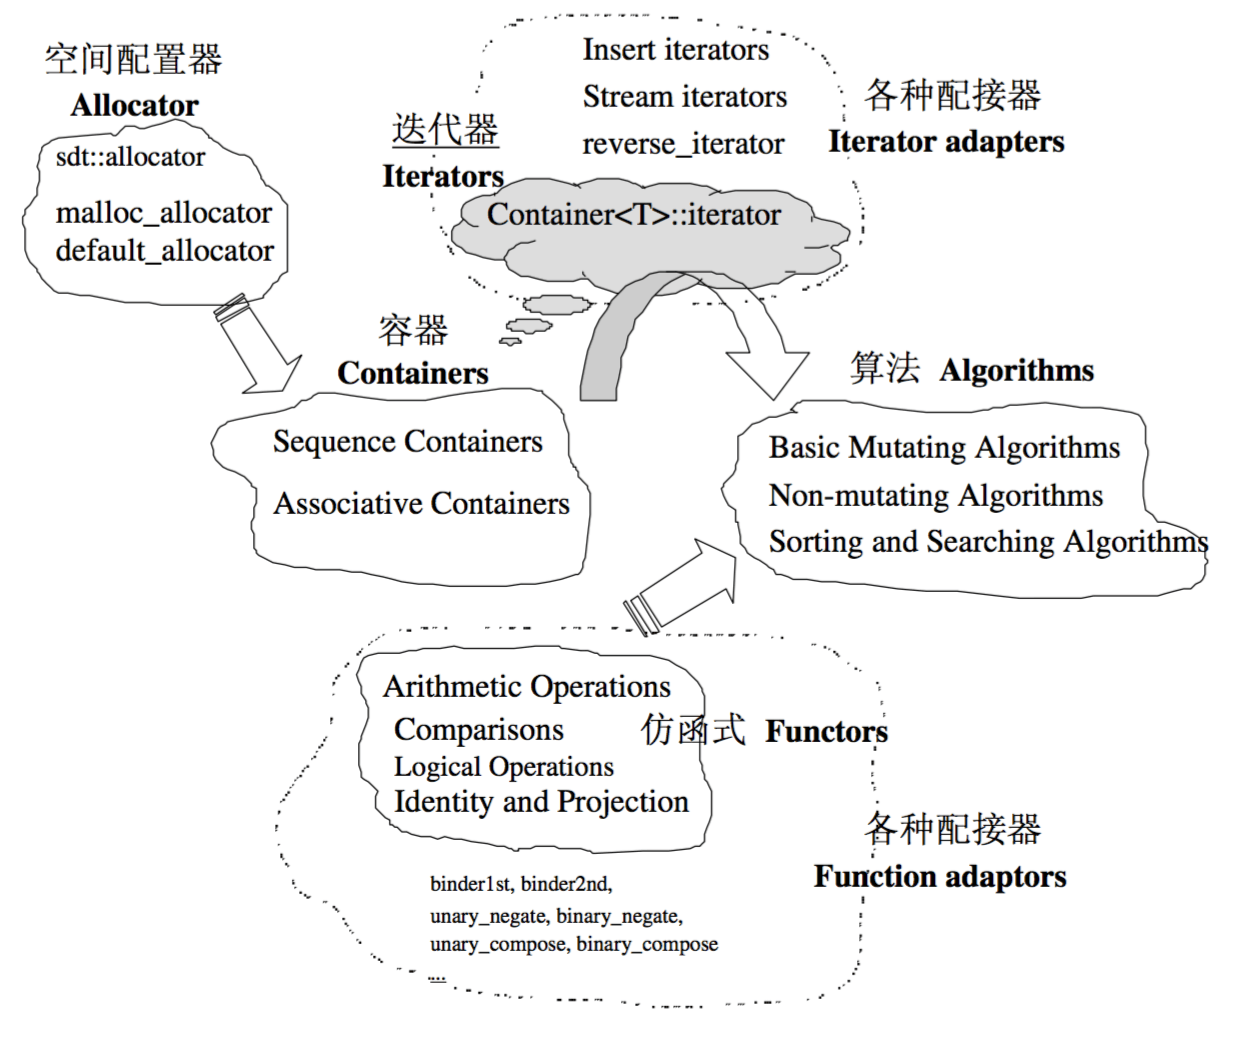
\includegraphics[width=0.75\textwidth]{CppSTL.png}
	\caption{六大组件的交互关系}
\end{figure}

\subsection {容器}

一个容器就是一些特定类型对象的集合。STL 中容器分为两大类,序列式容器和关联式容器。

序列式容器(sequential container)为程序员提供了控制元素存储和访问顺序的能力。这种顺序不依赖于元素的值,而是与元素加入容器时的位置相对应。

除了序列式容器容器外,标准库还定义了三个序列式容器适配器:stack、queue和priority_queue。适配器是标准库中的一个通用概念,容器、迭代器和函数都有适配器。本质上,一个适配器是一种机制,能使某种事物的行为看起来像另外一种事物一样。

和序列式容器对应的是关联容器(associative-container),关联容器中的元素是按关键字来保存和访问的。关联容器支持高效的关键字查找和访问,STL有两个主要的关联容器:map 和 set。

\subsubsection {顺序容器}

最简单的 STL 顺序容器就是 vector。Vector 只是一个拥有扩展功能的数组。

\begin{Code}
vector<int> v(10, 0);
int elements_count = v.size();
bool is_nonempty_ok = !v.empty();
\end{Code}

这里 V 包含了10 个 int 整数,初始化为0。Vector 最常使用的特性就是获取容器size,有两点要注意:首先,size() 函数返回的值是无符号的,这点有时会引起一些问题。其次,如果你想知道容器是否为空,把 size() 返回值和0比较不是一个好的做法。最好使用 empty() 函数,因为不是所有容器都能在常量时间内返回自己的大小,而且你绝不应该为了确定链表中至少包含一个节点元素就对一条双链表中的所有元素计数。

另一个 vector 中经常使用的函数是 push_back。Push_back 函数永远向 vector 尾部添加一个元素,容器长度加 1。当需要调整 vector 的大小时,使用 resize() 函数。如果在使用了 resize() 后又用了 push_back(),那新添加的元素就会位于新分配内存的后面,而不是被放入新分配的内存当中。

\begin{Code}
v.resize(15);
for(int i = 1; i < 5; i++) {
	v.push_back(i*2);
	//把元素写入下标值[15..20), not [10..15)
}
\end{Code}

向 vector 添加数据的最简单方式是使用 push_back()。但是,万一我们想在除了尾部以外的地方添加数据呢?Insert函数可以实现这个目的,往 vector 中插入一个元素:

\begin{Code}
vector<int> v(10,0);
v.insert(1, 42);    // Insert value 42 after the first
\end{Code}

从第二个(下标为1的元素)往后的所有元素都要右移一位,从而空出一个位置给新插入的元素。如果你打算添加很多元素,那多次右移并不可取——明智的做法是单次调用 insert(),指明插入数据的空间范围。

\begin{Code}
vector<int> v1(3,0);
vector<int> v2{1,2,3};
v1.insert(v1.begin(), v2.begin(), v2.end());
\end{Code}

还应该记住另一个非常重要的事情:当 vector 作为参数传给某个函数时,实际上是复制了这个 vector(也就是值传递)。在不需要这么做的时候创建新的 vector 可能会消耗大量时间和内存。实际上,很难找到一个任务需要在传递 vector 为参数时对其进行复制。所以,最好使用引用传递:

\begin{Code}
void some_function(const vector<int>& v) { 
	// Read only!
}
void some_function(vector<int>& v) { 
	// Can be Modified!
}
\end{Code}
此外,要知道我们可以创建任何类型的 vector,通过 vector 创建二维数组,最简单的方式就是创建一个存储 vector 元素的 vector。
\begin{Code}
int N=5, M=10;
vector< vector<int> > Matrix(N, vector<int>(M, -1));
\end{Code}
我们创建了一个 N * M 的矩阵,并用 -1 填充所有位置上的值。

erase()函数从指定容器删除指定位置的元素或某段范围内的元素,如果是删除指定位置的元素时,返回值是一个迭代器,指向删除元素下一个元素;如果是删除某范围内的元素时:返回值也表示一个迭代器,指向最后一个删除元素的下一个元素。

删除 vector 中指定的某个元素值(删除一个元素后导致后面所有的元素会向前移动一个位置):
\begin{Code}
vector<int> array = {1,2,6,6,7,8};
for (vector<int>::iterator itor = array.begin(); itor != array.end(); itor++)
{
	if (*itor == 6) {
		array.erase(itor);
		itor--;
	}
}
// 1,2,7,8
\end{Code}
其他的一些函数:
\begin{enumerate}
	\item   clear():清空 vector,使其包含 0 个元素,成为空容器。
	\item   capacity():返容器占用的内存空间,注意和v.size()的区别(空间的分配和size的关系);
	\item   pop_back():删除尾部的数据,size -= 1;
	\item   c.at(index):传回索引为index的数据,如果index越界,抛出out_of_range异常。
	\item   c.front():返回第一个数据。
	\item   c.back():传回最后一个数据,不检查这个数据是否存在。
\end{enumerate}

很多时候大量删除数据,或者通过使用reserver(),结果vector占有的空间远远大于实际的需要,这时候需要压缩vector到它的实际大小。在 C++11 中已经提供了shrink_to_fit()函数实现vector的压缩。
\begin{Code}
std::vector<int> v(1000,1);              // v.capacity()=1000
v.erase(v.begin(), v.begin()+v.size()/2);// v.capacity()=1000
v.shrink_to_fit();                       // v.capacity()=500
\end{Code}
(空间增长策略:按照容器现在容量的一倍进行增长。vector容器分配的是一块连续的内存空间,每次容器的增长,并不是在原有连续的内存空间后再进行简单的叠加,而是重新申请一块更大的新内存,并把现有容器中的元素逐个复制过去,然后销毁旧的内存。这时原有指向旧内存空间的迭代器已经失效,所以当操作容器时,迭代器要及时更新。)

\subsubsection {关联容器}

关联容器用来支持高效的关键字查找和访问,其中的元素是按照关键字来保存和访问的。与之相对,顺序容器中的元素是按它们在容器中的位置来顺序保存和访问的。两个主要的关联容器类型是 map 和 set:

 map中的元素是一些关键字-值对(key-value)对:关键字起到索引的作用,值则表示与索引相关联的数据。
 set中每个元素只包含一个关键字,set支持高效的关键字查询操作——检查一个给定关键字是否在 set 中。

标准库提供了8个关联容器,体现在三个不同的维度:

1. 或者是一个 map,或者是一个 set;

2. 允许关键字重复,或者不允许;

3. 按照顺序保存元素,或者无序保存。

具体情况如下表:

\begin{enumerate}
\item 定义关联容器

定义 map 必须指明关键字类型和值类型,而定义一个set时,只需要指明关键字类型。
\begin{Code}
map <string, size_t> word_count; // 空容器
set <string> exclude = {"the", "but", "and"}; // 列表初始化
map <string, string> authors = {{"Joyce", "James"},
	{"Austen", "Jane"}};
\end{Code}
对于有序容器,关键字类型必须定义元素比较的方法。默认情况下,标准库使用关键字类型的 < 运算符来比较两个关键字。

无序容器使用关键字类型的 == 运算符来比较元素,它们还使用一个hash<key_type>类型的对象来生成每个元素的哈希值。标准库为内置类型定义了 hash 模板,还为一些标准库类型,如 string 定义了hash。但是我们不能直接定义关键字类型为自定义类类型的无序容器。因为不能直接使用哈希模板,必须提供我们自己的 hash 模板版本。

\subitem pair类型

标准库类型 pair 是用来生成特定类型的模板,创建一个 pair 时必须提供两个类型名,pair的数据成员将具有对应的类型。
\begin{Code}
pair<string, string> anon{"James", "Joyce"};
pair<string, vector<int>> line;
\end{Code}
与其他标准库类型不同,pair的数据成员是 public 的,两个成员分别命名为 first 和 second,使用普通的成员访问符来访问它们。
\begin{Code}
cout << anon.first << anon.second;
\end{Code}

\item 关联容器操作

关联容器的类型有如下三个:
\begin{table}[hbp]
	\begin{tabular}{|c|l|}
		\hline
类型& 解释\\\hline
key_type &对应容器类型的关键字类型 \\ \hline
 mapped_type& map 关键字关联的类型 \\ \hline
 value_type& 对于 set,与 key_type 相同,对于map,为 pair<const key_type, mapped_type> \\ \hline
	\end{tabular}
\end{table}

解引用关联容器迭代器时,得到一个类型为容器的 value_type 的值的引用。对于map而言,value_type 是一个 pair 类型,其 first 成员保存 const 的关键字,second 成员保存值。

\begin{Code}
map<int, string> test{{1, "1"}};
auto iter = test.begin();
cout << iter->first << ", " << iter->second << endl;
// iter->first = 2;         // 关键字类型是 const 的
iter -> second = "2";
cout << iter->first << ", " << iter->second << endl;
\end{Code}

与不能改变 map 的关键字一样,一个 set 中的关键字也是 const 的,可以用一个 set 迭代器来读元素的值,但不能修改。

通常不对关联容器使用泛型算法,因为关键字是 const 这一特性意味着不能将关联容器传递给修改或者重排容器元素的算法(这类算法往往需要向元素写入值)。关联容器可用于只读取元素的算法。

\subitem \textbf{添加元素}

关联容器的 insert 成员向容器添加一个元素或一个元素的范围。insert 有两个版本,分别接受一对迭代器,或者是一个初始化器列表。注意,由于map 和 set 包含不重复的关键字,因此插入一个已经存在的元素对容器没有任何影响。
\begin{Code}
vector <int> ivec = {4,3,2,1,1,2,3,4};
set<int> set2;
set2.insert(ivec.cbegin(), ivec.cend());
// set2 = {1, 2, 3, 4} 有四个元素
\end{Code}
对 map 进行 insert 操作时,必须记住元素类型是 pair,一般在insert 参数列表中创建一个 pair:
\begin{Code}
map<string, int> word_count;
word_count.insert({"or", 1});
word_count.insert(make_pair("the", 1));
word_count.insert(pair<string, int>("and", 1));
word_count.insert(map<string, int>::value_type("text", 1));
\end{Code}
\subitem \textbf{检测 insert 的返回值}

insert 返回的值依赖于容器类型和参数,对于不包含重复关键字的容器,添加单一元素的 insert返回一个 pair,告诉我们插入操作是否成功。pair 的 first 成员是一个迭代器,指向具有给定关键字的元素,second 成员是一个 bool 值,指出元素是插入成功还是已经存在于容器中。
\begin{Code}
map<string, int> word_count;
word_count.insert({"or", 1});
auto ret = word_count.insert(make_pair("or", 1));
if(!ret.second){
	ret.first->second += 1;
}
// {"or", 2}
\end{Code}
我们要知道这里 ret 的类型为:
\begin{Code}
pair<map<string, int>::iterator, bool> 
\end{Code}
对允许重复关键字的容器,接受单个元素的 insert 操作返回一个指向新元素的迭代器,这里无需返回一个 bool值,因为 insert 操作总是向这类容器中加入一个新元素。

\subitem \textbf{删除元素}

关联容器定义了三个版本的 erase,与顺序容器一样,可以通过传递给 erase 一个迭代器删除一个元素或者一个迭代器对删除一个元素范围。这两个版本和顺序容器的操作类似,指定的元素被删除,返回 void。

此外,关联容器提供额外的 erase 操作,接受一个 key_type 参数,此版本删除所有匹配给定关键字的元素(如果存在的话),返回实际删除的元素的数量。对于保存不重复关键字的容器,erase返回值总是0或者1。

\subitem \textbf{map 的下标操作}

map 和 unordered_map 容器提供了下标运算符和一个对应的at函数。set类型不支持下标,因为set中没有与关键字相关联的值。也不能对 multimap 或 unordered_multimap 进行下标操作,因为这些容器中可能有多个值与一个关键字相关联。

如果关键字不在 map 中,会为它创建一个元素并插入到 map 中,关联值将进行值初始化。由于下标运算符可能插入一个新元素,我们只可以对非 const 的map使用下标操作。
\begin{Code}
map<string, int> word_count;
word_count["test"];
word_count["give"] = 1;
// word_count: {{give, 1},{test, 0}}
\end{Code}
上面最后一句执行的操作如下:

1. 在 word_count 中搜索关键字为 give 的元素,未找到;
2. 将一个新的关键字-值对插入到 word_count 中,关键字是一个 const string,保存 give,值进行初始化为0;
3. 提取出新插入的元素,并将值 1 赋予它。

对一个 map 进行下标操作时,会获得一个 mapped_type 对象。

\subitem \textbf{ 访问元素}

关联容器提供多种查找一个指定元素的方法,如果只关心一个特定元素是否已在容器中, find 是最佳选择。

|    操作     |   含义   |
|----------- |----------|
|  c.find(k) | 返回一个迭代器,指向第一个关键字为 k 的元素,若 k 不在容器中,则返回尾后迭代器 |
| c.count(k) | 返回关键字等于k的元素的数量,对于不允许重复关键字的容器,返回值永远是0或1    |
| c.lower_bound(k) | 返回一个迭代器,指向第一个关键字不小于 k 的元素| 
| c.upper_bound(k) | 返回一个迭代器,指向第一个关键字大于 k 的元素 |
| c.equal_range(k) | 返回一个迭代器 pair,表示关键字等于 k 的元素的范围。若 k 不存在,pair 的两个成员均等于 c.end() |

在一个不允许重复关键字的关联容器中查找一个元素是一件很简单的事情,元素要么在容器中,要么不在。但对于允许重复关键字的容器来说,过程更为复杂:容器中可能有很多元素具有给定的关键字。如果一个 multimap 或 multiset 中有多个元素具有给定关键字,则这些元素在容器中会相邻存储。
\begin{Code}
multimap<string, int> authors{{"Alain", 1}, {"Alain", 2}, {"Alain", 3}};
string search_item("Alain");
auto iter = authors.find(search_item);
auto entries = authors.count(search_item);
while(entries){
	cout << iter->second << endl;
	iter++;
	entries--;
}
\end{Code}
此外,可以用 lower_bound 和 upper_bound 来解决此类问题。 
\begin{Code}
for(auto beg = authors.lower_bound(search_item), end = authors.upper_bound(search_item);
beg != end; beg++){
	cout << beg->second << endl;
}
\end{Code}
\end{enumerate}

\subsection {迭代器}

迭代器提供对一个容器中的对象的访问方法,并且定义了容器中对象的范围。迭代器就如同一个指针。事实上,C++的指针也是一种迭代器。但是,迭代器不仅仅是指针,因此你不能认为他们一定具有地址值。例如,一个数组索引,也可以认为是一种迭代器。

迭代器有各种不同的创建方法。程序可能把迭代器作为一个变量创建。一个STL容器类可能为了使用一个特定类型的数据而创建一个迭代器。作为指针,必须能够使用操作符类获取数据。还可以使用其他数学操作符如++操作符用来递增迭代器,以访问容器中的下一个对象。如果迭代器到达了容器中的最后一个元素的后面,则迭代器变成past-the-end值。使用一个past-the-end值得指针来访问对象是非法的,就好像使用NULL或为初始化的指针一样。

对于STL数据结构和算法,可以使用五种迭代器。下面简要说明了这五种类型:

 Input iterators 提供对数据的只读访问
 
 Output iterators 提供对数据的只写访问
 
 Forward iterators 提供读写操作,并能向前推进迭代器
 
 Bidirectional iterators提供读写操作,并能向前和向后操作
 
 Random access iterators提供读写操作,并能在数据中随机移动


\subsection {算法}

STL通过函数模板提供了很多作用于容器的通用算法,例如查找、插入、删除、排序等,这些算法均需要引入头文件<algorithm>。

所有的 STL 算法都作用在由迭代器 [first, last) 所标示出来的区间上,可以分为两大类:

 质变算法(mutating algorithms):运算过程中会更改区间内迭代器所指的元素内容,如分割(partition)、删除(remove)等算法
 非质变算法(nonmutating algorithms):运算过程中不会更改区间内迭代器所指的元素内容,如匹配(search),计数(count)等算法

所有泛型算法的前两个参数都是一对迭代器,通常称为first和last,用以标示算法的操作区间。注意,将无效的迭代器传给某个算法,虽然是一种错误,但不保证能够在编译期间被捕捉出来。


\subsection {高效、安全使用 STL}

都是STL,可能写出来的效率相差几倍,所以要掌握写出高效 STL 代码的技巧。

\subsubsection {建立指针的容器}

当对象很大时,建立指针的容器而不是对象的容器,主要基于下面两个原因:

1. STL基于拷贝的方式的来工作,任何需要放入STL中的元素,都会被复制;这也好理解,STL工作的容器是在堆内开辟的一块新空间,而我们自己的变量一般存放在函数栈或另一块堆空间中。如果复制的对象很大,由复制带来的性能代价也不小;对于大对象的操作,使用指针来代替对象能消除这方面的代价;

2. 只涉及到指针拷贝操作,没有额外类的构造函数和赋值构造函数的调用。

下面例子:
\begin{Code}
	vector <BigObj> vt1;
	vt1.push_back(myBigObj);
	vector <BigObj* > vt2;
	vt2.push_back(new BigObj());
\end{Code}


不过要注意:

1. 容器销毁前需要自行销毁指针所指向的对象;否则就造成了内存泄漏;
2. 使用排序等算法时,需要构造基于对象的比较函数,如果使用默认的比较函数,其结果是基于指针大小的比较,而不是对象的比较;

\subsubsection {用区间成员函数}

尽量用区间成员函数代替单元素操作,使用区间成员函数有以下好处:

1. 更少的函数调用
2. 更少的元素移动
3. 更少的内存分配

例:将v2后半部的元素赋值给v1:

\begin{Code}
for (vector<Widget>::const_iterator ci = v2.begin() + v2.size() / 2;
ci != v2.end();
++ci)
v1.push_back(*ci);
// 使用区间成员函数assign()
v1.assign(v2.begin() + v2.size() / 2, v2.end());
\end{Code}

\subsubsection {避免 vector 频繁内存分配}

新增元素空间不够时,vector会进行如下操作:

1. 分配当前空间的两倍空间;

2. 将当前元素拷贝到新的空间中;

3. 释放之前的空间;

4. 将新值放入新空间指定位置;

如果预先知道空间的大小,预先分配空间(使用 reserve,或者定义 vector 时指明大小)避免了重新分配空间和复制的代价;注:reserve()只是修改了容量,并非大小,向vector中增加元素还是需要通过push_back加入;

\subsubsection {关联容器还是有序 vector}

对一些阶段性的操作:做一系列插入、完成之后,后续操作都是查询。使用vector有以下优势:

1. 因为可以对vector排序,关联容器带来的有序优势丧失;
2. 使用二分法查找的前提下,查询算法对连续的内存空间的访问要快于离散的空间;

\subsubsection {仿函数还是函数指针}

在仿函数(functor, 函数对象)的方式中,内联有效,而作为函数指针时,一般编译器都不会对函数指针指向的函数进行内联;即使指定了inline;

\begin{Code}
inline bool doubleGreater(double d1, double d2)
{
	return d1 > d2;
}
vector<double> v;
sort(v.begin(), v.end(), doubleGreater);
\end{Code}

这个调用不是真的把doubleGreater传给sort,它传了一个doubleGreater的指针。更好的方式是使用仿函数:

\begin{Code}
struct myclass {
	inline bool operator() (int i, int j) {
		return (i<j);
	}
} myobject;

sort(v.begin(), v.end(), myobject);
\end{Code}

\subsubsection {其它小条款}

1. 用empty()
 代替size()来检查是否为空。对于list,size()会遍历每一个元素来确定大小,时间复杂度 o(n),线性时间;而empty总是保证常数时间;
 
2. 尽量用成员函数代替同名的算法。基于效率考虑,成员函数知道自己这个容器和其他容器有哪些特有属性,能够利用到这些特性;而通用算法不可以;此外对于关联容器,成员函数find基于等价搜索,而通用算法find基于相等来搜索;可能导致结果不一样;

\subsection{参考}  

《STL 源码剖析》  

[标准模板库(STL)使用入门(上)](http://blog.jobbole.com/87586/)
  
[标准模板库(STL)使用入门(下)](http://blog.jobbole.com/88310/) 

[防止缓冲区溢出](http://www.ibm.com/developerworks/cn/security/buffer-defend/index.html)

[高效使用 STL](https://segmentfault.com/a/1190000002932246)  

[cplusplus:vector::reserve](http://www.cplusplus.com/reference/vector/vector/reserve/)
  
[C++ STL轻松导学](http://morningspace.51.net/resource/stlintro/stlintro.html)  

《C++ Primer》 11章:关联容器  

\section{C++编译和编译器}

\subsection{C++ 编译器工作原理}

简单地说,一个编译器就是一个程序,它可以阅读以某一种语言(源语言)编写的程序,并把该程序翻译成一个等价的、用另一种语言(目标语言)编写的程序。

C/C++编译系统将一个程序转化为可执行程序的过程包含:

\begin{itemize}
\item 预处理(preprocessing):根据已放置的文件中的预处理指令来修改源文件的内容。
\item 编译(compilation):通过词法分析和语法分析,在确认所有指令都是符合语法规则之后,将其翻译成等价的中间代码表示或汇编代码。
\item 汇编(assembly):把汇编语言代码翻译成目标机器指令的过程。
\item 链接(linking):找到所有用到的函数所在的目标文件,并把它们链接在一起合成为可执行文件(executable file)。
\end{itemize}


\subsubsection{预处理} 

预处理器是在程序源文件被编译之前根据预处理指令对程序源文件进行处理的程序。预处理器指令以\# 号开头标识,末尾不包含分号。预处理命令不是C/C++语言本身的组成部分,不能直接对它们进行编译和链接。C/C++语言的一个重要功能是可以使用预处理指令和具有预处理的功能。C/C++提供的预处理功能主要有文件包含、宏替换、条件编译等。

\begin{enumerate}
\item 文件包含

预处理指令 \# include 用于包含头文件,有两种形式:\# include <xxx.h>,\# include "xxx.h"。

尖括号形式表示被包含的文件在系统目录中。如果被包含的文件不一定在系统目录中,应该用双引号形式。在双引号形式中可以指出文件路径和文件名。如果在双引号中没有给出绝对路径,则默认为用户当前目录中的文件,此时系统首先在用户当前目录中寻找要包含的文件,若找不到再在系统目录中查找。

对于用户自己编写的头文件,宜用双引号形式。对于系统提供的头文件,既可以用尖括号形式,也可以用双引号形式,都能找到被包含的文件,但显然用尖括号形式更直截了当,效率更高。

\item 宏替换

\textbf{宏定义}:一般用一个短的名字代表一个长的代码序列。宏定义包括无参数宏定义和带参数宏定义两类。宏名和宏参数所代表的代码序列可以是任何意义的内容,如类型、常量、变量、操作符、表达式、语句、函数、代码块等。

宏定义在源文件中必须单独另起一行,换行符是宏定义的结束标志,因此宏定义以换行结束,不需要分号等符号作分隔符。如果一个宏定义中代码序列太长,一行不够时,可采用续行的方法。续行是在键入回车符之前先键入符号\\,注意回车要紧接在符号\\之后,中间不能插入其它符号,当然代码序列最后一行结束时不能有\\。

预处理器在处理宏定义时,会对宏进行展开(即\textbf{宏替换})。宏替换首先将源文件中在宏定义随后所有出现的宏名均用其所代表的代码序列替换之,如果是带参数宏则接着将代码序列中的宏形参名替换为宏实参名。宏替换只作代码字符序列的替换工作,不作任何语法的检查,也不作任何的中间计算,一切其它操作都要在替换完后才能进行。如果宏定义不当,错误要到预处理之后的编译阶段才能发现。

\item 条件编译

一般情况下,在进行编译时对源程序中的每一行都要编译,但是有时希望程序中某一部分内容只在满足一定条件时才进行编译,如果不满足这个条件,就不编译这部分内容,这就是\textbf{条件编译}。

条件编译主要是进行编译时进行有选择的挑选,注释掉一些指定的代码,以达到多个版本控制、防止对文件重复包含的功能。if, \# ifndef, \# ifdef, \# else, \# elif, \# endif是比较常见条件编译预处理指令,可根据表达式的值或某个特定宏是否被定义来确定编译条件。

此外,还有 \# pragma 指令,它的作用是设定编译器的状态或指示编译器完成一些特定的动作。
\end{enumerate}
\subsubsection{编译} 

编译过程的第一个步骤称为词法分析(lexical analysis)或扫描(scanning),词法分析器读入组成源程序的字符流,并且将它们组织成有意义的词素的序列,对于每个词素,词法分析器产生一个词法单元(token),传给下一个步骤:语法分析。

语法分析(syntax analysis)或解析(parsing)是编译的第二个步骤,使用词法单元来创建树形的中间表示,该中间表示给出了词法分析产生的词法单元流的语法结构。一个常用的表示方法是语法树(syntax tree),树中每个内部结点表示一个运算,而该结点的子结点表示该运算的分量。

接下来是语义分析(semantic analyzer),使用语法树和符号表中的信息来检测源程序是否和语言定义的语义一致。

在源程序的语法分析和语义分析之后,生成一个明确的低级的或者类机器语言的中间表示。接下来一般会有一个机器无关的代码优化步骤,试图改进中间代码,以便生成更好的目标代码。

\subsubsection{汇编} 

对于被翻译系统处理的每一个C/C++语言源程序,都将最终经过这一处理而得到相应的目标文件。目标文件中所存放的也就是与源程序等效的目标机器语言代码。目标文件由段组成,通常一个目标文件中至少有两个段:代码段和数据段。

\begin{itemize}
\item 代码段:该段中所包含的主要是程序的指令。该段一般是可读和可执行的,但一般却不可写。
\item 数据段:主要存放程序中要用到的各种全局变量或静态的数据。一般数据段都是可读,可写,可执行的。
\end{itemize}

\subsubsection{链接} 

链接程序的主要工作就是将有关的目标文件彼此相连接,也即将在一个文件中引用的符号同该符号在另外一个文件中的定义连接起来,使得所有的这些目标文件成为一个能够按操作系统装入执行的统一整体。主要有静态链接和动态链接两种方式:

\begin{itemize}
\item 静态链接:在链接阶段,会将汇编生成的目标文件.o与引用到的库一起链接打包到可执行文件中,程序运行的时候不再需要静态库文件。
\item 动态链接:把调用的函数所在文件模块(DLL)和调用函数在文件中的位置等信息链接进目标程序,程序运行的时候再从DLL中寻找相应函数代码,因此需要相应DLL文件的支持。  
\end{itemize}

这里的库是写好的现有的,成熟的,可以复用的代码。现实中每个程序都要依赖很多基础的底层库,不可能每个人的代码都从零开始,因此库的存在意义非同寻常。本质上来说库是一种可执行代码的二进制形式,可以被操作系统载入内存执行。库有两种:静态库(.a、.lib)和动态库(.so、.dll),所谓静态、动态是指链接方式的不同。

静态链接库与动态链接库都是\textbf{共享代码}的方式。如果采用静态链接库,程序在运行时与函数库再无瓜葛,移植方便。但是会浪费空间和资源,因为所有相关的目标文件与牵涉到的函数库被链接合成一个可执行文件。此外,静态库对程序的更新、部署和发布也会带来麻烦。如果静态库更新了,所有使用它的应用程序都需要重新编译、发布给用户。

动态库在程序编译时并不会被连接到目标代码中,而是在程序运行是才被载入。不同的应用程序如果调用相同的库,那么在内存里只需要有一份该共享库的实例,规避了空间浪费问题。动态库在程序运行是才被载入,也解决了静态库对程序的更新、部署和发布页会带来麻烦。用户只需要更新动态库即可,增量更新。

此外,还要注意静态链接库中不能再包含其他的动态链接库或者静态库,而在动态链接库中还可以再包含其他的动态或静态链接库。

\subsubsection{简单的例子} 

下面是一个保存在文件 helloworld.cpp 中一个简单的 C++ 程序的代码:
\begin{Code}
    /* helloworld.cpp */
    #include <iostream>
    int main(int argc,char *argv[])
    {
        std::cout << "hello, world" << std::endl;
        return 0;
    }
\end{Code}

用下面命令编译:
\begin{Code}
    $ g++ helloworld.cpp
\end{Code}

编译器 g++ 通过检查命令行中指定的文件的后缀名可识别其为 C++ 源代码文件。编译器默认的动作:编译源代码文件生成对象文件(object file),链接对象文件和 libstd c++ 库中的函数得到可执行程序,然后删除对象文件。由于命令行中未指定可执行程序的文件名,编译器采用默认的 a.out。

\begin{enumerate}

\item 预处理

\textbf{选项 -E} 

使 g++ 将源代码用编译预处理器处理后不再执行其他动作。下面的命令预处理源码文件 helloworld.cpp,并将结果保存在 .ii 文件中:

\begin{Code}
    ➜  ~  g++ -E helloworld.cpp -o helloworld.ii
    ➜  ~  ls | grep helloworld
    helloworld.cpp
    helloworld.ii
    ➜  ~  wc -l helloworld.ii
       38126 helloworld.ii
\end{Code}
helloworld.cpp 的源代码,仅仅有六行,而且该程序除了显示一行文字外什么都不做,但是,预处理后的版本将超过3万行。这主要是因为头文件 iostream 被包含进来,而且它又包含了其他的头文件,除此之外,还有若干个处理输入和输出的类的定义。

\item  编译

\textbf{选项 -S} 

指示编译器将程序编译成汇编代码,输出汇编语言代码而后结束。下面的命令将由 C++ 源码文件生成汇编语言文件 helloworld.s,生成的汇编语言依赖于编译器的目标平台。

\begin{Code}
    g++ -S helloworld.cpp
\end{Code}

\item  汇编

\textbf{选项 -c}

 用来告诉编译器将汇编代码(.s文件,或者直接对源代码)转换为目标文件,但不要执行链接。输出结果为对象文件,文件默认名与源码文件名相同,只是将其后缀变为 .o。

\begin{Code}
    ➜  ~  g++ -c helloworld.s
    ➜  ~  ls |grep helloworld.o
    helloworld.o
\end{Code}

\item  链接

加载相应的库,执行链接操作,将对象文件(.o,也可以直接将原文件)转化成可执行程序。

\begin{Code}
    ➜  ~  g++ helloworld.o -o helloworld.o
    ➜  ~  ./helloworld.o
    hello, world 
\end{Code}
\end{enumerate}

\subsubsection{参考} 
 
[详解C/C++预处理器](http://blog.csdn.net/huang_xw/article/details/7648117)  

[Compiling Cpp](http://wiki.ubuntu.org.cn/Compiling_Cpp)
  
[C++静态库与动态库](http://www.cnblogs.com/skynet/p/3372855.html)  

[高级语言的编译:链接及装载过程介绍](http://tech.meituan.com/linker.html)  
  
[编译原理](http://www.cnblogs.com/pipicfan/archive/2012/07/10/2583910.html) 
 



\chapter{Robocup2d足球的入门}
\section{2D仿真足球的简介}
1997年是人工智能领域发展中的重要一年,该年5月IBM的机器人“深蓝”击败了人类国际象棋冠军,揭开了人工智能领域的崭新一页。同年首届Robocup比赛及会议在日本名古屋举行,迈出了实现机器人足球击败人类足球世界冠军这一梦想的第一步。

Robocup(Robot World Cup),即机器人世界杯足球赛,它涉及人工智能、机器人学、通讯、传感等诸多领域的前沿研究和技术集成。是在动态不确定环境下对人工智能的考验,是培养信息、自动化领域科技人才的重要手段。而2D仿真足球就是机器人足球世界杯仿真组比赛中的一个类别,是在二维空间角度对足球赛的一种仿真。由于不需要较多的资金投入,仿真组的比赛是目前参赛队伍最多的比赛。



\section{2D仿真足球的仿真过程}
Robocup 2d仿真足球比赛的仿真平台软件rcsoccersim(RoboCup Soccer Simulator),该平台包括一个简单的仿真机器人例程rcssclient,仿真比赛监视程序rcssmonitor,仿真比赛重播程序rcssslogplayer和最主要的仿真比赛服务器程序rcssserver。

比赛时,各参赛队将自己编写好的仿真足球程序加载到仿真平台上去,让其在rcsoccersim提供的虚拟场地自主的进行比赛。比赛采用Client/Server模式,简称C/S结构,每个Client模块只允许控制一名机器人,Client之间不允许直接进行通信,只能通过Server服务器才能进行通信,Server服务器实际上控制着整个比赛。

Server与Client之间的通信都是通过UDP/IP协议来实现的,所以Client的开发和运行环境只需支持UDP/IP协议即可。Server服务器包括两个程序:Soccer Server和Soccer Monitor。其中,Monitor是比赛监视器,显示虚拟场地;Server可以与多个Monitor相连在多个显示器上同时显示比赛情况。客户端程序分为以下四种类型,其中球员智能体,智能体教练,训练师智能体被统称为足球智能体。
\begin{figure}[H]
	\centering 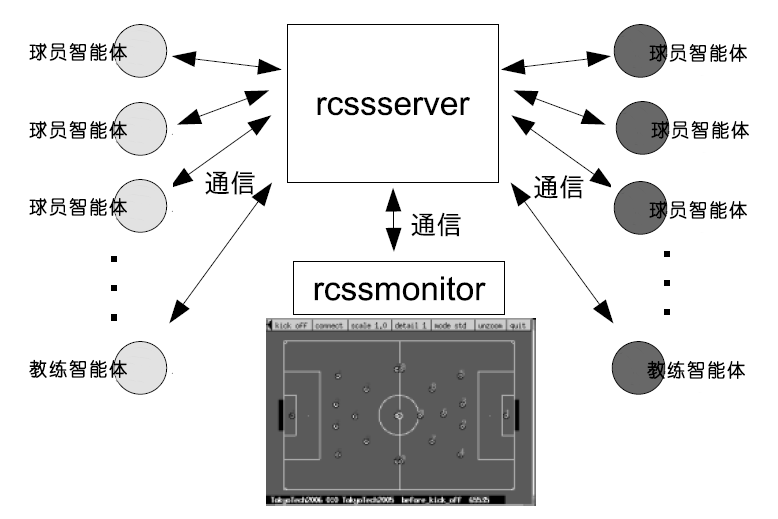
\includegraphics[width=0.65\textwidth]{server.png}
	\caption{2D仿真模拟的结构}
\end{figure}

\begin{itemize}
	\item \textbf{球员智能体}
	
	可以控制场上的球员。不但能得到成段的信息,只有得到部分的、包含噪声的信息。
	\item \textbf{教练智能体}
	
	能够获得关于对象的完整的位置信息。能给予球队意见,但不能直接控制球员。它在比赛过程中使用。
	\item \textbf{训练器智能体}
	
	它除了具有教练的能力,还可以控制同一场比赛中的裁判。它不能在比赛过程中使用。所以也被称为离线教练。
\end{itemize}
\section{2D仿真足球的特点}

通过上面的介绍,可以看到,作为一个试验平台,这套仿真比赛平台提供了一个很好的
全分布的、包括合作与对抗的多主体实时环境,非常有挑战性。其具体特点如下:
\begin{itemize}
	\item \textbf{分布式多主体团队合作和对抗}  所有客户端程序分别控制场上的一名球员或教练,
	自主决策,分布运行,队友之间有合作,对手之间有对抗
	\item \textbf{动态、实时、不确定环境}  在服务器端,整个系统按照100 毫秒的周期运转,所有
	球员都必须按照这个周期运行,意味着球员的所有决策都必须实时完成,由于多主体
	的存在,环境在动态的转变,无法预知(这也被称为“不透明转换”[Stone 1998])。
	\item \textbf{感知和行为异步}  由于比赛时间以周期为单位离散,感知和行为就无法同步,所以
	光靠传统人工智能方法使用感知来激发行动是远远不够的
	\item \textbf{球员能力受限}  场上所有球员能力都是参照真实球员有所限制的,如体力、加速度、
	最大速度、惯性等
	\item \textbf{视觉受限}  每个球员的视觉都是局部的,收到球员视角、和视距的限制,也就是说
	球员在任何时刻都只能获得一部分球场上的信息。这就给球员正确分析场上形势,进
	而产生决策带来了困难
	\item \textbf{通讯受限}  球员之间的通讯环境具有单信道、窄带宽等特点,即每队球员公用一条
	信道,每个球员一个周期内只能“听”到队友一条消息,而且信道容量很有限(缺省
	为10 字节)。这样,现有的一些团队合作理论就很难直接应用,因为目前大部分合作
	理论前提都是要求通讯是及时的、完全的
	\item \textbf{多噪声源}  为了真实模拟实际比赛,仿真世界里球员感知和动作都带有噪声,使得
	球员既无法精确地感知世界也不能完全按照它的意图影响世界
	\item \textbf{连接不可靠}  平台网络连接使用UDP/IP,不确保所有信息的正确及时,在网络繁忙
	时一些信息甚至会丢失,这也体现了比赛环境的不确定性,球员程序必须能够适应这
	一环境。
\end{itemize}

\section{基本模型与基本命令}
\subsection{时间模型}
rcssserver是一个离散时间仿真。定期更新其中的状态,对象的位置将仅在该时间更新。这在rcssmonitor中被显示为这个比赛仿真的时间。信息是定期周期更新的,但是,每个智能体的发送和接收消息是与该周期异步完成的。

通常情况下,场内的状态被认为是100毫秒更新一次。因此,理想情况下,rcssmonitor将以每秒10帧更新显示。

\subsection{物理模型}
rcssserver的物理模型与现实世界有很大的不同。例如,地面和物体之间的摩擦系数不考虑,速度衰减率被速度参数所取代。这是因为,它不是现实世界的完全仿真平台,rcssserver被设计为能够流畅运行多智能体仿真环境的仿真平台。



\subsection{球场坐标系}
rcssserver内部的坐标系统使用左手坐标系统. rcssmonitor领域的正确查看方式是,以原点场为中心,向右为X轴正方向,向下是Y轴正方向。它角度的规定也是遵守这样的规则。换句话说,从场中心,右方为0度起算线,左侧方向是180度,向上为-90度,向下为90度。当进行角度计算时,任何时候正方向都是顺时针方向。

如下图所示,该区域的大小是长105米、宽64米。场中心为原点,图形的每个边角的坐标值如图所示。
\begin{figure}[htb]
	\centering 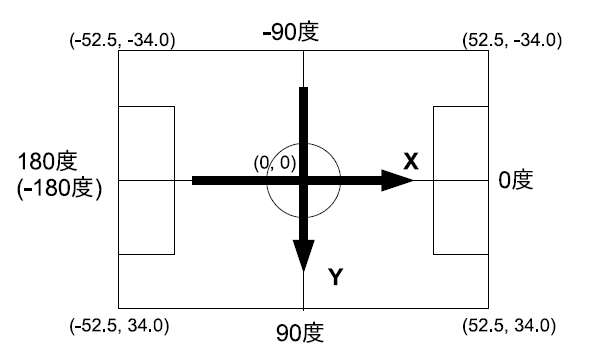
\includegraphics[width=0.65\textwidth]{playground.png}
	\caption{球场坐标}
\end{figure}
\subsubsection{播放系统的坐标}

球员智能体的坐标系统与rcsserver的坐标系统略有不同。在左侧的球队与rcssserver的坐标系是完全一样的,而右边的则与rcssserver的坐标系完全相反。也就是说,一球场为中心,左方为X轴正方向,上方为Y轴正方向,角度将被反转。虽然很容易混乱,但是“敌人的方向是X轴正方向”会帮助您很好的记忆。

\subsubsection{训练智能体及教练智能体的坐标系}
训练智能体及教练智能体使用和rcssserver一样的坐标系。
\subsection{裁判}
rcssserver进行了足球比赛裁判功能的内置,它的判定十分明确,甚至不会错过一毫米。然而,它没法确定恶意犯规的。

裁判是自动的,会根据球员和球的位置,相应地更改运行模式,重置球员和球。它会通知所有的智能体新的球场状态。
规则尽可能接近到现实的人类足球的规则。

在大多数情况下,这里的裁判我们也可以认为它仅仅是用来开球的程序。
在没有人类的强迫干预的情况下,内置的裁判无法判断是否犯规的。
如果在正式比赛时,监视器出现了以下情况,就视为犯规: 

·如果一支球队将球围住,以至于对方队员无法踢到球; 
·如果球门被许多球员挡住,以至于对方无法进球(如将球员排成人墙挡住球门);
·如果一支球队试图挡住对方球员的运动; 

另外,任何其它的被技术委员会认定的违反公平竞赛的行为,也都可以被视为犯规。


\section{平台的搭建}
首先在个人工作电脑上正确安装ubuntu操作系统,并能连接网络。

搭建过程:

(1)系统准备

sudo apt-get install nautilus-gksu

把“管理员打开选项”添加到右键菜单中

sudo apt-get install nautilus-open-terminal
把终端添加到右键菜单中

sudo apt-get install rar unrar p7zip
安装解压缩程序

(注意这几个程序需要注销后才能生效)

sudo apt-get install build-essential
安装gcc编译器

(2)安装必要的库、解析器、图像化界面
(3)平台安装
首先下载源

rcssserver-14.0.3.tar.gz  
rcssmonitor-14.1.1.tar.gz   
rcssslogplayer-14.0.1.tar.gz

以server安装为例,进入终端,依次键入

-> tar xf rcssserver-14.0.3.tar.gz   //解压文件,会出现一个同名的文件夹

->cd rcssserver-14.0.3         //进入文件夹

-> ./configure             //配置库等一系列东西

-> make

sudo make install                 //必须root装

sudo ldconfig                    //修改软件数据库 缓存

rcssmonitor和rcssslogplayer的安装过程同上。
注意,如果在进行操作时,提示权限不够,可以输入:chomd 777 configure

形成自动化脚本如下:\footnote{适用于ubuntu 14.04,其他系统自行更改库的名字}

\begin{Codex}[label=install.sh]
#!/bin/bash
#更新中科大源 貌似是最新的14.04
sudo cp sources.list /etc/apt/sources.list
sudo apt-get update

#安装相应的包
sudo apt-get install -y build-essential libboost-all-dev flex 
sudo apt-get install -y libqt4-dev libxpm-dev libaudio-dev libxt-dev
 libpng-dev libglib2.0-dev libfreetype6-dev libxrender-dev libxext-dev
  libfontconfig-dev libxi-dev

#独立编译bision
tar -zxvf bison-2.7.1.tar.gz
cd bison-2.7.1
./configure
make
sudo make install
cd ..
sudo ldconfig

#独立编译sever
tar -zxvf rcssserver-15.2.2.tar.gz
cd rcssserver-15.2.2 
./configure --with-boost-libdir=/usr/lib/x86_64-linux-gnu
make
sudo make install
cd ..

#独立编译player(也可安装soccerwindow2)
tar -zxvf rcsslogplayer-15.1.0.tar.gz
cd rcsslogplayer-15.1.0
./configure --disable-gl --with-boost-libdir=/usr/lib/x86_64-linux-gnu
make
sudo make install
cd ..

#独立编译monitor
tar -zxvf rcssmonitor-15.1.0.tar.gz
cd rcssmonitor-15.1.0 
./configure --with-boost-libdir=/usr/lib/x86_64-linux-gnu
make
sudo make install
cd ..
sudo ldconfig
\end{Codex}
\section{球队上场}
正如之前所说的,每一个球员和教练都是一个程序client,理论上我们只要启动server和球员程序就可以仿真了。
但是如果想一下子启动12个都带有不同配置的程序就没有那么简单了,这里我们通常使用shell来完成这些工作,实现
比赛和测试的自动化。

\subsection{Server的配置启动}
启动server非常简单,在终端中输入rcssserver就可以启动程序。在默认情况下,server只启动6000一个端口,
也就意味着一般只能启用一个rcssserver,进行一场比赛。但是实际上可以突破这个限制,进行多线程的测试,这里
就不赘述了,请参见中科大Autotest自动化测试脚本。\footnote{http://github.com/USTC-ro/AutoTest}

Rcssserver还有很多参数可以设置,配置文件在 ~/.rcssserver/server.conf 
主要配置有:
\begin{Codex}[label=server.conf]
#修改下面的两个参数 可以设置log
# server::game_log_compression
server::game_log_compression = 0
# server::text_log_compression
server::text_log_compression = 0

#调整下面两个参数 可以切换有无点球 
# server::nr_extra_halfs  
/* Number if extra-time periods in a game if it is drawn */
#server::nr_extra_halfs = 0
server::nr_extra_halfs = 2

# server::nr_normal_halfs
/* Number of normal halfs in a game */
#server::nr_normal_halfs = 0
server::nr_normal_halfs = 2
\end{Codex}

\subsection{分布式测试脚本的编写(单个球员启动)}
一般在比赛中经常使用这种脚本,该脚本大多是由官方提供的,我们只需要进行基本的配置修改就可以上线了。
这也是最基本、最简单的脚本,其他复杂的脚本都由此衍生。
\begin{Codex}[label=start]
#!/bin/sh
#这里接受服务器参数
HOST=$1
BASEDIR=$2
NUM=$3

# 下面这个代码,是链接动态库的代码,Yushan底层都需要添加
if [ -z "$LD_LIBRARY_PATH" ]
then
	LD_LIBRARY_PATH=.:./src
else
	LD_LIBRARY_PATH=.:./src:$LD_LIBRARY_PATH
fi
export LD_LIBRARY_PATH

#这里开始配置球队的信息
teamname="IEU2016"

player="./IEU2016_Player"
coach="./IEU2016_Coach"

config="./data/player.conf"
config_dir="./data/formations-dt"
coach_config="./data/coach.conf"

opt="--player-config ${config} --config_dir ${config_dir}"
opt="${opt} -h ${HOST} -t ${teamname}"

coachopt="--coach-config ${coach_config}"
coachopt="${coachopt} -h ${HOST} -t ${teamname}"

cd $BASEDIR
#注意到,这里只启动了一个球员
case $NUM in
    1)
        $player $opt -g
        ;;
    12)
        $coach $coachopt
        ;;
    *)
        $player $opt
        ;;
esac

\end{Codex}

\subsection{单机测试脚本的编写(全部球员启动)}
一般在自己测试的过程中,我们往往由于设备的限制,需要在本地上线所有球员和教练,形成脚本如下。
该脚本是Yushan对Agent脚本的简化,减去了太多不常用的配置。

\begin{Codex}[label=start.sh]
#!/bin/bash
#=======================================================
# Agent2D-3.1.0 start script
# RoboCup2D @ Anhui Unversity of Technology
# Bugs or Suggestions please mail to guofeng1208@163.com
#=======================================================


if [ -z "$LD_LIBRARY_PATH" ]
then
	LD_LIBRARY_PATH=.
else
	LD_LIBRARY_PATH=.:$LD_LIBRARY_PATH
fi

export LD_LIBRARY_PATH


host="localhost"
port=6000
coach_port=6002
teamname="YuShan"

player="./YuShan_Player"
coach="./YuShan_Coach"

config="./data/player.conf"
coach_config="./data/coach.conf"
config_dir="./data/formations-dt"
log_dir="./log"

opt="--player-config ${config} --config_dir ${config_dir}"
debugopt="--player-config ${config} --config_dir ${config_dir} --offline_logging --debug --debug_server_connect --debug_server_logging --log_dir ${log_dir}"

coachopt="--coach-config ${coach_config} --use_team_graphic on --debug --debug_server_connect --log_dir ${log_dir}"

sleeptime=0.5
posnum=0
count=12

#这里想对单机脚本来说,多了一些配置,实际上不影响启动
usage()
{
cat << EOF
Usage: $0  [options]
    
Options:
	-help               Show help infomation
	-h      (IP)        Special server host address
	-p      (port)      Special the server port number of player
	-t      (Name)      Special teamname
	-c      (number)    Special player amount(start with 1)
	-n      (number)    Special player position number(Not uniform)
EOF
}


if [ $# -eq 1 -a "$1" = "-help" ]
then
    usage
    exit 0
fi


while getopts "h:p:t:c:n:" flag
do
    case "$flag" in
    h)
        host=$OPTARG
    ;;
    p)
        port=$OPTARG
        coach_port=$((port+2))
    ;;
    t)
        teamname=$OPTARG
    ;;
    c)
        count=$OPTARG
    ;;
    n)
        posnum=$OPTARG
    ;;
    *)
    	echo "Error cmdline option"
    	usage
    	exit 1
    esac
done


opt="${debugopt} -h ${host} -p ${port} -t ${teamname}"
coachopt="${coachopt} -h ${host} -p ${coach_port} -t ${teamname}"


# the limit of core dump file size 
ulimit -f unlimited


if [ $posnum -ne 0 ]
then
	case $posnum in
	1)
		${player} ${opt} -g -n $posnum &
	;;
	12)
		${coach} ${coachopt}  &
	;;
	*)
		${player} ${opt} -n $posnum  &
	;;
	esac
	
	exit 0
fi

i=1
# 这里使用循环语句,可以上线所有球员	
while [ ${i} -le ${count} ]
do
	case ${i} in
	1)
		echo "team $teamname: Start Player $i"
		${player} ${opt} -g &
	;;
	12)
		echo "team $teamname: Start Coach"
		${coach} ${coachopt} &
	;;
	*)
		echo "team $teamname: Start Player $i"
		${player} ${opt} &
	;;
	esac

	sleep $sleeptime
	i=$((i+1))
done

exit 0

\end{Codex}
\section{一些工具的使用}


\subsection{soccerwindow2}
soccerwindow2是一个播放器,用于观看之前的比赛录像,从而可以研究球队在进攻与防守上可以改进的地方,同时soccerwindow2中的Debug功能还拥有调试功能,move dialog功能有球队定向调试的功能,通过Debug调试我们可以逐个周期观察各个球员要执行的动作和实际执行的动作,从而可以知道在某个周期自己的代码是否起到作用,通过move dialog可以观察球队定向修改的效果。

打开soccerwindow2,点击file,即可打开要观看的日志文件(.rcg),在观看比赛录像时可以进行一些必要的设置,点击Ctrl+V即可视图设置,进行Canvas、Show、Object上的设置

Canvas:

如下图,其中Scale可用于调节整个球场的大小;lines可将球场网格化。



Show:

如下图,其中Anonymous Mode是匿名模式,点上后,即可隐藏队名、队标;

点上Score Board、player、ball……即可显示记分榜、球员、球等信息;

点上View Area和Body Shadow即可显示球员的视角和球员的后方,其中Body Shadow选项还可以通过球员身后 


Object:

如下图,其中ball size和player size可以调节球和队员的大小;

focus可以选择视场集中的地方;

player selection可以选择是否将视场集中于某个球员。



Debug功能

打开soccerwindow2,点击菜单栏中的Debug即可打开Debug选项,如下图:



选择上方一栏的球员号码,点击菜单栏上方左边的打开按钮,导入相应球员的日志文件,即可观察到各个球员在每周期内某一动作动作链评估出的动作,以及评估处该动作的相关信息。点击左侧的按钮即可选择不同的动作类型。

Move Dialog

同时利用soccerwindow2选择在某一特定场景下,重新开始两支球队的比赛,也就是可以进行相同条件下不同队伍的比赛,即可以实现对一支球队定向修改效果的观察,点击Monitor,选择move dialog,即可打开相应界面,如下图:



选择相应的日志文件,打开球队比赛录像,选择自己想要重新开始的周期,点击保存按钮,然后重新开始跑经过特定修改的两支球队,重新打开move dialog界面,点击最下方的send按钮,即可为球队设置初始环境,点击kick off开始比赛。


\subsection{fedit}

Fedit2是2d仿真中的阵型编辑器,用于比赛队伍的基本队形编辑,设置队员的本位点。利用fedit2还可以绘制自己球队的delaunay三角形。

绘制delaunay三角形的方法

打开fedit2,界面如下图:



鼠标拖动球在球场内移动,当到达自己的预计点位时,点击上方工具栏最右边的红点,该点位即被记录,同时在球场的上下对称方向的对称点位也被记录,重复移动球的位置,最终将得到己方球队的delaunay三角形,点击工具栏右数第三个按钮该阵型即被记录。

绘制己方阵型的方法

打开fedit2,如上图,在一个已经绘制好的delaunay三角形上,当球位于一点时,鼠标拖动球员移动,方法如上,当为所有球员确定点位时(本位点),点击工具栏的保存按钮,该阵型即被保存。(注意上述文件保存的路径全为英文路径)

\subsection{队标的制作}
工具:
1. FireWorks  
2. ACD Photo Editor 
3. convert 

1、准备自己喜欢的图片(可以是JPG、PNG等常用的格式) 

2、用FireWorks 打开图片,然后选择[文件]-[图像预览]。 

3、在[文件]中设置像素宽为192,高为48。 

4、在[选项]中设置 “格式”为BMP8, 
“调色板”接“近网页最合适”或“最合适”(自己预览哪一种更好); 
在右边的方框内输入“32”,再勾选上[抖动] 100% , 
最后点取右下边的[导出]按钮,得到BMP格式的文件。 这一步最关键; 

5、用ACD Photo Editor打开FireWorks导出得到的01.BMP图片, 
打开[调整]-[色深]选项,改“256色(8位)”为“16色(4位)” 
然后保存为*.BMP图片。 

6、最后一步用convert打开刚才的BMP位图,然后转化成XPM格式即可。   

\chapter{Yushan底层开发手册}

Agent2D是秋山英久博士(日本)开发的一套基于UVA底层的仿真2D底层,汇集了球队底层基本动作和大部分基础问题的解决方案。球队开发伊始,它可以用作参考模板。在后续开发过程中,也可以对其进行编辑、调整。

中国安徽工业大学Yushan队对Agent2D的代码结构和编译方法上进行了优化,形成了编译效率高、可操作性强的底层。IEU队的代码就是基于YushanBase上开始开发的。
\section{框架分析与源码结构}

在Agent2d\_base上进行了结构调整,优化了一系列的makefile。(感谢Yushan\_GF学长)YS的版本rcsc库开放,更利于学习者学习;可执行文件与源码分开,减少赛场失误。

修改过后的类库和球队代码结构如下:
\begin{figure}[htb]
	
\includegraphics{rcsc.png}
	\caption{rcsc库的结构及作用}
\end{figure}


\begin{figure}[H]
	%\usepackage{float}
	
\includegraphics{src.png}
	\caption{src的结构及作用}
\end{figure}

\begin{itemize}
	\item body*.cpp/.h	球员原子动作
	\item bhv*.cpp/.h	组合动作(原子动作特定组合,为实现某种目的),策略,战术
	\item neck*		颈的动作,用于提高信息精度
	\item view*		视角的选用策略
\end{itemize}
\section{开发工具与使用}
欲立其事,必先利其器。在Yushan架构下的2D代码的开发过程中,我们寻找到了一些工具和方法来方便编码和
调试。工具的熟练使用也是我们能够高效工作的基础,希望大家能够熟练的使用下面的工具。
\subsection{代码编辑与编译}
\subsubsection{QT简介}
IDE是×××,

QT是一个跨平台C++图形用户界面应用程序开发框架。它既可以开发GUI程序,也可以开发非GUI程序,比如控制台工具和服务器。QT是面向对象的框架,使用特殊的代码生成扩展以及一些宏,易于扩展,允许组件编程。

QT在编辑上的优势。。。。
\subsubsection{使用QT管理yushan底层}

\subsection{代码调试与分析}

\subsubsection{日志分析}
日志是我们调试代码的一种重要手段,我们之前在命令行下面变成的时候,通常使用输出日志文件的方式来调试代码。
这种可以快速定位程序分支执行情况和错误发生的地方。秋山在Agent2D的开发中,也同样使用了这种方法,并留下了
非常好、非常完善的日志类供开发者使用。
在YushanBase中启动调试功能非常简单,只需修改 data/player_config.conf 下如下参数即可:

秋山教授在soccerwindow2中同样开发了将日志信息可视化的功能,让日志文件可以在soccerwindows中更直观的展示
出来,方便开发者使用,使用方法如下:

当然我们也可以针对自己的程序编写自己的日志记录,比如在调试一个小功能的时候,并不想调用庞大的底层中dlog,
我们可以自己编写文件输入输出代码,来记录调试自己的功能。
\subsubsection{动态调试}
当然日志记录并不能解决所有的问题,比如,在我们在测试中出现了bug,需要复盘曾经出现过的现象,进行动态调整代码
的时候便行不通了。Agent2D在这里也提供了类似蓝鹰DynamicDebug的功能,被称作OfflineMode。
这个功能,通过记录比赛时的全部信息并输出为文件,然后在程序启动调试模式之后,将这些以前记录下的数据“伪装”成服务器发播的信息,供Client程序使用,以实现复盘重现、动态调试的效果。

实际上这种动态调试并不是真正的动态调试,只能一种非实时的程序调试。不过对于我们来说这已经足够了,有了这些东西
我们可以清晰的了解程序的运行情况,尽情的去除bug了!!

offlineMode的启动和使用方法如下:
\subsection{版本控制}

\subsubsection{Git简介} 

Git是一个开源的分布式版本控制/软件配置管理软件。Git可以用于1、管理编程源代码:个人项目、集体项目;2、合作编写文档并用 Git 管理;3、配合 Github/Gitcafe/... 等代码托管网站, 轻松实现代码同步、参与开源项目;等等。Git尤其适合1、个人小项目管理;2、联系紧密的小项目组合作开发;3、多人协作大中型开源项目管理 (如 Github 托管的各类项目)。

Git 的工作流(workflow)设计,以及它对分支(branch)操作的支持十分优秀
Git 由一系列的小工具组成,配合使用完 成工作任务。如: git add, git commit, git reset, git checkout, git remote, git bisect, git diff ......


\subsubsection{Git使用实例}
以 /tmp/tmp 目录作为项目的工作目录, 在其中创建一个 README 纯文本文件, 并使用 Git。

第一步:初始化 Git 版本库
1. 进入工作目录(如,使用cd),并输入
\begin{Code}
	git init
	初始化空的 Git 版本库于 /home/wt/.git/
\end{Code}
2. 初始化配置 :
\begin{Code}
	git config --global user.name "Wu Tong"
	git config --global user.email "1159559828@qq.com"
\end{Code}
查看当前工作树状态:
\begin{Code}
	git status
	位于分支 master
	无文件要提交,干净的工作区
	随时运行 git status 即可查看当前状态, 工作情况尽在掌握之中。
\end{Code}

第二步:编辑文件
3. 创建一个新文件并写入内容:
\begin{Code}
	touch README
	echo "Hello World!" > ./README
	查看文件内容:
	cat ./README
\end{Code}

第三步:添加到暂存区

4. 添加 README 文件至暂存区:
\begin{Code}
	git add ./ README
\end{Code}


5. 进行初始提交:
\begin{Code}
	git commit -m 'First Commit'
\end{Code}




\section{开发心得}

\subsection{学习优秀代码}
作为一个2D的初学者,最初一般都是从学习别人的代码开始的。2D项目发展到现在,我们已经有很多优秀的代码可以学习。比如Helios08年的代码,2011年国内各个球队公开的代码,以及各个公布底层的代码。其中都包含大量的优秀代码值得大家学习。

但是对于一个如此庞大的项目学起来自然是很费力的,所以一定的方法是有必要的。在2年多的时间里,我们2014届的队员大部分的时间都在学习别人的代码,也总结了一些学习的方法,希望对大家有帮助。

\subsubsection{框架学习}
在学习之前,我们必须要对自己要学习的东西有一定的了解,也就是说如果我们想深入的学习这些东西,我们到底要从哪里下手,这就是需要了解清楚整体程序的框架。这里以YushanBase为例,进行讲解。

上一节中我们已经了解了基本的代码的结构和功能,如此繁多的模块是如何组织在一起的。任何一个程序都会从main()开始,我们的机器人程序也不例外。程序运行的流程图如下。
	\begin{figure}[H]
		\centering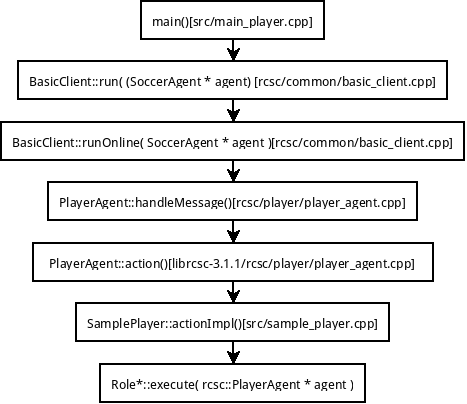
\includegraphics[width=0.65\textwidth]{run.png}	
		\caption{ agent 流程图}
	\end{figure}


毋庸置疑,任何代码的执行都是从main函数开始的,agent也不例外。
每个agent的main函数首先设置和判断一下signal,然后转入BasicClient
类的run ()方法启动agent。接着进入BasicClient的runOnline ()方法启动在
线Agent, runOnline () 方法调用PlayerAgent类的handleMessage ()方法
处理获得的信息,处理完之后handleMessage () 方法调用在同一个类中
的方法action()进行动作决策。在action()方法依次进行actionImpl() (body
动作决策) ,doArmAction() (手臂动作决策),doViewAction() (视觉决策),
doNeckAction() (颈部动作决策)以及communicationImpl () (通信决策) 。
这里要注意一下, PlayerAgent类的actionImpl() 是一个纯虚函数,也就是说
实际的动作决策是在其子类SamplePlayer的方法actionImpl()中完成的。这就是整个Yushan架构运行的流程,每个周期都会往复运转。

PlayerAgent类的actionImpl() 是一个纯虚函数,所以我们从它的子类SamplePlayer的方法actionImpl() 开始看起。方法actionImpl() 首先根据该agent的球员号码创建该agent对应的球员角色,然后当比赛模式为playon的时候调用该类球员角色的execute () 方法进行该类球员角色的body动作决策。当然, actionImpl() 还进行了许多非playon模式下的agent决策。

球员角色的基类是SoccerRole,派生了8个子类RoleCenterBack,RoleCenterForward,RoleDefensiveHalf……(在src的8个以role开头的头文件中定义),分别对应于场上的前锋,中场,后卫等等。球队策略中是根据agent的号码生成该agent对应的球员角色。在现实的比赛中,这些球员角色的区别是很明显的(比如说前锋活跃在中前场,经常射门,后卫活跃在后场,经常大脚解围等),那么在代码中,这些区别是如何实现的呢?这些区别agnet2D的底层为我们实现了一些,但是大部分还是靠我们自己编写代码来实现,也就涉及到各种模型的建立。

上面说到了,agent的body动作决策实际上交给了该类agent对应的球员角色,那么我们现在来看看每类角色到底是如何进行决策的。在agent2D的底层源代码中,八类角色的决策代码几乎是一模一样的(守门员除外),都是先判断自己是否是持球队员,如果是,则按照bhv_basic_offensive_kick.cpp文件中的hv_BasicOffensiveKick::execute()方法进行决策,如果不是,则按照bhv_basic_move.cpp文件中的hv_BasicMove::execute()方法进行跑位或者截球等决策。这一部分就是我们工作的重心,我们要修改这8个文件,使球队能够按照我们的决策来进行比赛。这里大家重点注意一下,agent2d底层已经为搭建了一个决策框架:作者将整个球场划分为10个区域,每类角色的球员可以在这10个区域中进行单独决策,以适应我们的决策需要。
\subsubsection{模型学习}
所谓模型,就是球赛中一些战术或动作的处理方法(包括理论和代码)。通常一个队伍会建立一个模型库\footnote{参考第五章},以收集需要开发的功能和基本思路,以使球队有完整的技术路线。所以真正的技术一般都会体现在这一部分,也就是说这里才是比赛中真正较量的地方。作为一个初学者,我们一般都先学习其他人的模型开始的。

这里以一个简单的学习Helios2008边后卫和中后卫的防守运动为例子,讲解如何学习前人的模型。首先比较一下下面两个代码\footnote{由于篇幅限制已去掉注释,copyright by Helios} 。

\begin{Codex}[label=bhv_side_back_defensive_move.cpp]
bool
Bhv_SideBackDefensiveMove::execute( PlayerAgent * agent )
{
	dlog.addText( Logger::ROLE,
	__FILE__": Bhv_SideBackDefensiveMove" );

	if ( Bhv_BasicTackle( 0.85, 50.0 ).execute( agent ) )
	{
		agent->debugClient().addMessage( "SB:Def:Tackle" );
		return true;
	}
	
	if ( doIntercept( agent ) )
	{
		return true;
	}
	
	if ( doAttackBallOwner( agent ) )
	{
		dlog.addText( Logger::ROLE,
		__FILE__": attack to ball owner" );
		return true;
	}
	
	if ( doEmergencyMove( agent ) )
	{
		return true;
	}
	
	doNormalMove( agent );
	return true;
	
}
\end{Codex}

\begin{Codex}[label=bhv_center_back_defensive_move.cpp]
bool
Bhv_CenterBackDefensiveMove::execute( PlayerAgent * agent )
{
	dlog.addText( Logger::TEAM,
	__FILE__": Bhv_CenterBackDefensiveMove" );
	
	if ( Bhv_BasicTackle( 0.85, 50.0 ).execute( agent ) )
	{
		agent->debugClient().addMessage( "CB:Def:Tackle" );
		return true;
	}
	
	if ( doIntercept( agent ) )
	{
		return true;
	}
	
	if ( doGetBall( agent ) )
	{
		return true;
	}
	
	doNormalMove( agent );
	return true;
	
}
\end{Codex}

比较这两个代码我们可以看到不同角色的球员策略大不相同。边后卫采取的是比较激进的策略,进行攻击对手和紧急补位;而中后卫采取的是getball的策略形成压制势力,防止对方突破。这里就可以看出一个模型只有用在一个正确的位置才能发挥其作用。这里面提到的几种防守的解决方案都是防守中可取的一些方法,下面对其攻击持球者的模型进行分析。

\begin{Codex}[label=bhv_side_back_defensive_move.cpp]
bool
Bhv_SideBackDefensiveMove::doAttackBallOwner( rcsc::PlayerAgent * agent )
{
	const rcsc::WorldModel & wm = agent->world();
	
	const int mate_min = wm.interceptTable()->teammateReachCycle();
	const int opp_min = wm.interceptTable()->opponentReachCycle();
	
	const AbstractPlayerObject * fastest_opp = wm.interceptTable()
						->fastestOpponent();
	
	if ( mate_min < opp_min )
	{
		dlog.addText( Logger::ROLE,
		__FILE__": doAttackBallOwner() ball owner is teammate" );
		return false;
	}
	
	if ( ! fastest_opp )
	{
		dlog.addText( Logger::ROLE,
		__FILE__": doAttackBallOwner() no opponent" );
		return false;
	}
	
	const Vector2D opp_trap_pos = wm.ball().inertiaPoint( opp_min );
	
	const Vector2D home_pos = Strategy::i().getPosition( wm.self().unum() );
	const PositionType position_type = Strategy::i().
			getPositionType( wm.self().unum() );
	
	const MarkTable & mark_table = Strategy::i().markTable();
	const AbstractPlayerObject * mark_target = 
				mark_table.getTargetOf( wm.self().unum() );
	const AbstractPlayerObject * free_attacker = 
			static_cast< AbstractPlayerObject * >( 0 );
	
	if ( mark_target )
	{
		dlog.addText( Logger::ROLE,
		__FILE__": doAttackBallOwner() mark_target= %d (%.1f %.1f)",
		mark_target->unum(),
		mark_target->pos().x, mark_target->pos().y );
		
		//
		// find other free attacker
		//
		const AbstractPlayerCont::const_iterator o_end = wm.allOpponents().end();
		for ( AbstractPlayerCont::const_iterator o = wm.allOpponents().begin();
		o != o_end;
		++o )
		{
			const AbstractPlayerObject * marker = mark_table.getMarkerOf( *o );
			if ( marker ) continue; // exist other marker
			if ( (*o)->pos().x > mark_target->pos().x + 10.0 ) 
				continue; // no attacker
			if ( ( position_type == Position_Left
			&& (*o)->pos().y < mark_target->pos().y + 10.0 )
			|| ( position_type == Position_Right
			&& (*o)->pos().y > mark_target->pos().y - 10.0 )
			|| ( position_type == Position_Center
			&& std::fabs( (*o)->pos().y - mark_target->pos().y ) < 10.0 )
			)
			{
				free_attacker = *o;
				break;
			}
		}
	}
	
	if ( free_attacker )
	{
		dlog.addText( Logger::ROLE,
		__FILE__": doAttackBallOwner() exist free_ataccker= %d (%.1f %.1f)",
		free_attacker->unum(),
		free_attacker->pos().x, free_attacker->pos().y );
	}

	const double min_y = ( position_type == Position_Right
	? 2.0
	: -31.5 );
	const double max_y = ( position_type == Position_Left
	? -2.0
	: +31.5 );
	
	if ( fastest_opp == mark_target )
	{
		dlog.addText( Logger::ROLE,
		__FILE__": doAttackBallOwner() fastest_opp == mark_target, %d (%.1f %.1f) trap_pos=(%.1f %.1f)",
		mark_target->unum(),
		mark_target->pos().x, mark_target->pos().y,
		opp_trap_pos.x, opp_trap_pos.y );
		Rect2D bounding_rect( Vector2D( -50.0, min_y ),
		Vector2D( -5.0, max_y ) );
		if ( Bhv_GetBall( bounding_rect ).execute( agent ) )
		{
			agent->debugClient().addMessage( "SB:Def:GetBall(1)" );
			return true;
		}
	}

	if ( ! mark_target )
	{
		dlog.addText( Logger::ROLE,
		__FILE__": doAttackBallOwner() no mark target.
		 ball_owner=%d (%.1f %.1f) trap_pos=(%.1f %.1f)",
		fastest_opp->unum(),
		fastest_opp->pos().x, fastest_opp->pos().y,
		opp_trap_pos.x, opp_trap_pos.y );
		
		if ( opp_trap_pos.x < home_pos.x + 10.0
		&& ( std::fabs( opp_trap_pos.y - home_pos.y ) < 10.0
		|| ( position_type == Position_Left
		&& opp_trap_pos.y < home_pos.y )
		|| ( position_type == Position_Right
		&& opp_trap_pos.y > home_pos.y ) )
		)
		{
			dlog.addText( Logger::ROLE,
			__FILE__": doAttackBallOwner() no mark target. attack " );
			Rect2D bounding_rect( Vector2D( -50.0, min_y ),
			Vector2D( -5.0, max_y ) );
			if ( Bhv_GetBall( bounding_rect ).execute( agent ) )
			{
				agent->debugClient().addMessage( "SB:Def:GetBall(2)" );
				return true;
			}
		}
	}
	
	return false;
}
\end{Codex}
这个代码的条例非常清晰,首先进行盯人对象的选择,然后对盯人对象的分析,如果球员是最快的球员,就要去getball;同样是使用getball,边后卫的getball就目的性更明确,成功率增高了。
\subsection{优秀编码习惯}

条件编译

模块思想

版本控制


\section{常用的底层模型类}
\subsection{worldmodel}

\subsubsection{世界模型}
Librcsc 库中提供了 WorldModel 类,用来管理球员智能体的内部模型。 WorldModel类 Protected继承PlayerAgent 类的成员。如果 PlayerAgent 或它的派生类要获取运动场的信息,那就必须从 WorldModel 中获取。 WorldModel 类的成员中, SelfObject 类管理球员本身, BallObject 类用于管理球员和球信息,PlayerObject 类信息的容器也是其成员。其他的,包括当前时间、估计越位线也是他的成员,比如 InterceptTable 类来存储球的所有者判断信息。
\subsubsection{WorldModel访问}

%\begin{table}[htbp]
	\begin{tabular}{p{0.9\columnwidth}}
		\hline
		const GameTime \& getTime() const \\ 返回当前的仿真周期。\\
		\hline
		const GameMode \& getGameMode() const\\
		返回了比赛的当前运行模式的信息。\\
		\hline
		SideID getOurSide() const\\
		返回你的球队属于右或左侧信息。\\
		\hline
		const SelfObject \& self() const\\
		PlayerAgent本身的信息。\\
		\hline
		const BallObject \& ball() const\\
		球的信息\\
		\hline
		const PlayerCont \& teammates() const\\
		已明确球衣号码的队友\\
		\hline
		const PlayerCont \& unknownTeammates() const\\
		球衣号码不明的队友\\
		\hline
		const PlayerCont \& opponents() const\\
		已明确球衣号码的对方球员。\\
		\hline
		const PlayerCont \& unknownOpponents() const\\
		未知球衣号码的对方球员 \\
		\hline
	\end{tabular}
%\end{table}

%\begin{table}[htbp]
\begin{tabular}{p{0.9\columnwidth}}
	\hline
		const PlayerCont \& unknownPlayers() const\\
		身份无法识别球员。 \\
	\hline
		const PlayerPtrCont \& getTeammatesFromSelf() const\\
	将我方球员按照与自身距离由近及远排序。\\ 
	\hline
		const PlayerPtrCont \& getOpponentsFromSelf() const\\
		将对方球员按照与自身距离由近及远排序,也包含不能被识别的球员。\\
	\hline
		const PlayerPtrCont \& getTeammatesFromBall() const\\
		将我方球员按照与球d的距离由近及远排序。\\
	\hline
		const PlayerPtrCont \& getOpponentsFromBall() const\\
		将对方球员按照与球的距离由近及远排序,也包含不能被识别的球员。 \\
	\hline
		const PlayerObject * getOpponentGoalie() const\\
		返回对方守门员的指针。如果它不存在,则返回NULL。 \\
	\hline
		const PlayerObject * getTeammateNearestTo( const Vector2D \& point, const int count thr, double * dist to point ) const\\
		置信度count_thr下,返回距离point点最近的我方球员指针。若没有满足该条件的球员,则返回NULL。若dist_to_point不为NULL,则该球员到point之间的距离将会被保存(到dist_to_point中?) \\
	\hline
		const PlayerObject * getOpponentNearestTo( const Vector2D \& point,const int count thr, double * dist to point ) const\\
		类似上条,只是 对方球员版getTeammateNearestTo()。\\
	\hline
		const PlayerObject * getTeammate( const int unum ) const\\
		返回球衣号码为unum的我方球员指针,如果不存在,则返回NULL\\
	\hline
		const PlayerObject * getOpponent( const int unum ) const 
		类似上条,只是 对方球员版getTeammate()。\\
	\hline
		bool existKickableTeammate() const\\
		如果认定可能踢到球的我方球员为村内状态,返回true。 \\
	\hline
		bool existKickableOpponent() const\\
		对方球员版本existKickableTeammate() \\
	\hline
		const InterceptTable * getInterceptTable() const\\
		返回一个指向InterceptTable实体的const指针。 \\
	\hline
		int getDirCount( const AngleDeg \& angle ) const\\
		向angle方向观测最后一个周期。可作为场地区域的可信赖信息使用。(返回的整数究竟做什么用,没明白) \\
	\hline
		HeteroID getTeammateHeteroID( const int unum ) const\\
		返回球衣号码为unum的我方球员类型ID \\
	\hline

\end{tabular}
%\end{table}

\begin{tabular}{p{0.9\columnwidth}}
	\hline	
		const double \& getOffsideLineX() const\\
		估计越位线的横坐标值。\\
	\hline	
\end{tabular}	

\subsection{SelfObject}
\begin{tabular}{p{0.9\columnwidth}}
	\hline
		int unum() const; \\
		球衣号码\\
	\hline
		bool goalie() const; \\
		判断是否为守门员\\
	\hline
		const PlayerType \& playerType() const; \\
		异构球员的参数\\
	\hline
		cons Vector2D \& pos() const; \\
		位置坐标.\\
	\hline
		const Vector2D \& vel() const; \\
		速度.\\
	\hline
		const AngleDeg \& body() const; \\
		身体的绝对方向\\
	\hline
		const AngleDeg \& neck() const; \\
		头与身体朝向的相对角度\\
	\hline
		const AngleDeg \& face() const; \\
		头的绝对方向.\\
	\hline
		const ViewWidth \& viewWidth() const; \\
		当前的视角的大小\\
	\hline
		const GameTime \& catchTime() const; \\
		最后接/持球的时间\\
	\hline
		const double \& stamina() const; \\
		体能值\\
	\hline
		const double \& effort() const; dash \\
		与 Dash 命令效果相关联的体能值。\\
	\hline
		bool isKickable() const;\\
		能否踢到球。\\
	\hline
		const double \& kickRate() const kick \\
		实现 kick 命令的成效比例。它是由playerType() 的参数以及与球的位置关系来确定。\\
	\hline 


\end{tabular}

\begin{tabular}{p{0.9\columnwidth}}
	\hline	
		const double \& dashRate() const dash \\
		实现 dash 命令的成效比例。由playerType() 和 effort() 工作的参数来确定。 \\
	\hline
		const double \& tackleProbability() \\
		当前推算的成功概率。取[0,1]之间的实数值\\
	\hline	
\end{tabular}

\subsection{BallObject}
\begin{tabular}{p{0.9\columnwidth}}
	\hline
const Vector2D \& pos() const\\
位置坐标。 \\
\hline
int posCount() const\\
最后一个周期观测到的位置,作为可靠位置信息。 \\
\hline
const Vector2D \& rpos() const\\
从 SelfObject 出发的相对位置坐标。 \\
\hline
const Vector2D \& vel() const\\
速度。 \\
\hline
int velCount() const\\
最后一个周期观测到的速度,作为可靠速度信息使用。 \\
\hline
const double \& distFromSelf() const\\
与 SelfObject 之间的距离。 \\
\hline
const double \& distFromSelf() const\\
与 SelfObject 之间的绝对方向。 \\
\hline
Vector2D inertiaTravel( int cycle ) const\\
如果没有附加的加速度时,周期内的总移动向量\\
\hline
Vector2D inertiaPoint( int cycle ) const\\
如果没有附加的加速度时,循环后的位置。 \\
\hline
Vector2D inertiaFinalTravel() const\\
如果没有附加的加速度时,直到速度为0之前的总移动向量\\
\hline
Vector2D inertiaFinalPoint() const\\
如果没有附加的加速度时,速度变为0时的位置坐标。\\
\hline
\end{tabular}

\subsection{PlayerObject}
\subsubsection{PlayerAgent的访问}

Playeragent类包含WorldModel类和 ActionEffector类的成员变量。如果想从SampleAgent访问这些的话,可以使用如下成员函数。
\subsubsection{PlayerAgent成员}

\begin{tabular}{p{0.9\columnwidth}}
	\hline	
const WorldModel \& world() const;\\
返回一个WorldModel类实体的const引用/常量参照?。\\ 
	\hline
const ActionEffector \& effector() const;\\
返回一个ActionEffector类实体的const引用/常量参照?。\\
	\hline	
\end{tabular}



\subsubsection{PlayerObject 容器}

WorldModel存有PlayerObject作为其成员变量。对于观察到的多个球员(信息),将被存储在PlayerObject STL的容器中进行管理。

为了减少类型的量,PlayerObject容器通过typedef定义下列两种类型。

\begin{Code}
typedef std::list< PlayerObject > PlayerCont
typedef std::vector< PlayerObject * > PlayerPtrCont
\end{Code}

PlayerCont将用于存储PlayerObject的实例。对于需要频繁增删元素的情况,可使用std::list作为容器。

PlayerPtrCont用于保存PlayerObject的指针。该指针指向存储在PlayeCont的实例。为了实现快速调用,可使用的std :: vector。每当球员智能体的内部状态被更新时,即每当PlayerCont的内容要发生变化的时候, PlayerPtrCont就要进行重新调整。请注意,被存储的值是一个指针。


\subsection{InterceptTable}
InterceptTable类,从worldmodel内保留的信息预测出每名球员捕捉到球所必需的周期数,并将这一结果保存。在球员智能体决策时,可以参照捕捉到球的周期数,从而来判断哪只队伍的哪位球员正在持球。

\subsubsection{WorldModel 成员函数}
\begin{tabular}{p{0.9\columnwidth}}
	\hline	
int getSelfReachCycle() const\\
预测selfobject(球员智能体本身)捕获球的的周期数。\\ 
	\hline	
int getTeammateReachCycle() const\\
预测我方球员捕获球的周期数的最小值。 \\
	\hline	
int getOpponentReachCycle() const\\
预测对方球员捕获球的周期数的最小值。 \\
	\hline	
const PlayerObject * getFastestTeammate() const\\
预测最早捕获球的队友球员的指针*\\
	\hline	
const PlayerObject * getFastestOpponent() const\\
预测最早捕获球的对方球员的指针*\\
	\hline	
\end{tabular}



\subsection{ActionEffector}
相较于WorldModel,ActionEffector是用来记录球员智能体已执行或将要实施的动作,并推测其效果。例如,如果想要一边改变身体朝向,一边将头转向某一位置,那么,你必须掌握身体最终的朝向然后再转头才比较可行。这些可能尚未在rcssserver中得到体现,但是还是由ActionEffector来负责管理已经执行和将要实施的动作。

PlayerAgent类包含有一个ActionEffector类的成员变量。如果需要参考球员决策时使用的信息,就可以使用下面的成员函数。

\subsubsection{ActionEffector成员 }
\begin{tabular}{p{0.9\columnwidth}}
	\hline	
AngleDeg queuedNextMyBody()const; \\
在下一个周期中的身体方向。 \\
	\hline	
的Vector2D queuedNextMyPos()const; \\
下一个周期的位置坐标。 \\
	\hline	
的Vector2D queuedNextBallPos()const;\\ 
在下一周期中球的位置。 \\
	\hline	
的Vector2D queuedNextBallVel()const;\\ 
下一周期球的速度。 \\
	\hline	
AngleDeg queuedNextAngleFromBody(const Vector2D \& target) const; \\
从在下一周期中的目标位置与身体相对方向。 \\
	\hline	
ViewWidth queuedNextViewWidth()const; \\
下一个周期的视角。\\
	\hline	
\end{tabular}


\section{球队开发中的常用方法和模型}
底层的原子动作


%dointention	意图;\\
%doforcekick\\
%doshoot		射门(优先级最高);\\
%doprocess\\
%dopreprocess	如果被冻结(铲球失败等)只看(转脖子);开场前,进球后,位置如果不对,找位置;球员信息不准,观察(维护信息);\\
%非play_on模式:	free_kick 自由球; goal_kick 门球; indirect_free_kik 直接任意球; kick_in 角球; kick_off 开球;\\
%target_point, dist_thr, dash_power\\

\subsection{底层中的原子动作}
底层中存在一些原子动作,可以在server中直接注册动作的命令。
最常见的如下:doKick(),doDash(),doTurn(),doCatch(), doMove(),doTackle(),doTumNeck(),doChangeView(), doPointTo()等动作,这些方法属于PlayerAgent类,均可以使用agent->doKick()方法使用。其实以上的一系列动作在内部均使用ActionEffector类中的set系列方法来将每个动作及其参数转换为发送给server的命令。

以下以doKick为例说明其调用过程。

首先使用 Agent->doKick( power,dir),调用 PlayerAgent 中的 doKick 命令,此处的 power 和dir需要自己计算。
然后在doKick方法中对一些限制条件进行判断,如是否可踢,是否正在铲球状态等,
然后通过ActionEffector进行动作的设定,在ActionEffector中使用setICick(power,dir)方法, 该方法将参数进行规格化,转换成可直接发送给server的参数,最后通过 PlayerBodyCommand类将命令封装成可以发送给server的命令。

下面将详细说明下几个常用的命令:
\subsubsection{doKick}

\begin{Code}
	doKick( const double & power,const AngleDeg & rel_dir);
\end{Code}

该动作可以让球运动起來,是最基本的也是最常用的模型。
第一个参数是踢球的力量,该power不消耗体力值,第二个参数是踢球的角度。 使用该模型是,需要计算kick的power和kick的角度,这个根据踢球的目标点或者 目标方向计算。具体计算方法在下面的常用模型中将给出,一般先计算加速度,在根据加速 度计算其余两个参数。
当计算得到kick所需要的power和角度dir之后,
使用agent->doKick( power, rel_dir)即可发送命令,此处agent —般为传入的一个PlayAgent类型的参数。

\subsubsection{doDash}

\begin{Code}
	doDash(const double & power,const AngleDeg & rel_dir=0.0);
\end{Code}
该动作将一个球员加速,也就是球员跑动的命令。
该动作一般被封装在GotoPoint类中。
第一个参数power,该power消耗体力值。第二个参数为角度方向,默认值为0,即默认为只向身体内正前方加速。其实这里的dir在ActionEffector中经过一次转换,该转换
过程如下:
实际dir方向=自身身体方向+rcl_dir;
最后的方向可理解为相对身体的方向.

该模型的有两种使用方法。

第一种,单个方向的dash,使用一个参数,第二个参数使用默认参数0,即可使用单个方向((正前方)的dash。

使用方法如下:首先计算这次运动球员需要的dashpower,该dashpower —般使用范围理论上从0到100,但是实际上如果使用底层提供的计算dashpower的函数,则使用一个平均值在70左右的Power。Power值越大,加速的效果越好,但是由于体力值的总值固定,所以使用较大的dashPower会使球员体力降低过快,导致球员后期没有体力。所以体力
需要综合考虑。

agent->doDash(power)此方法将给球员提供一个单方向dash,球员向身体正前方移动。

第二种使用方法,多个方向的dash,为doDash()提供第二个参数,则可以实现向多个方向的dash。如发送doDash(power, 45.0)则球员使用power的大小,按照身体方向4 5度的方向进行移动。但第二个参数在发送时,需要进行处理,使用ServerParam中的一个函数 discretizeDashAngle()进行规格化处理。

在进行多个方向的Dash时,会产生效率问题,根据角度的不同,同样的power获得到的加速效果不一样.

\subsubsection{doTurn}

	\begin{Code}
	doTurn( const AngleDeg & moment)	
	\end{Code}
	
该动作让球员转身,当球员需要转身的时候使用该命令.

参数为转身的角度,该角度只是一个度量,可以这样理解,当前角度为0度,需要转到90度,则角度的参数为90度。如果当前身体角度为-10度,需要转到90度,则需要转动角度的参数应该为100度.

使用方法为 agent->doTurn(moment);

\subsubsection{doTackle}
\begin{Code}
	doTackle( const double & power_or_dir, const bool foul = false);
\end{Code}

铲球的命令,该命令让球员发—个铲球的动作。该命令一般封装在Bhv_BasicTackle.cpp中。

第一个参数为力量或者是角度,第二个参数决定该铲球是否为犯规铲球。默认的铲球是非犯规。第一个参数根据版本的不同而不同,当版本大于12时,铲球默认使用最大的力量,传入的第一个参数为铲球的角度。其他的情况是,传入的参数为铲球的力量。

和其他动作类似使用该方法是agent->doTackle( dir ,fasle )

使用该命令时,首先计算铲球的角度。然后确定是否使用犯规铲球,如果使用犯规铲球,则铲球失败后可能犯规。

\subsubsection{doPointto}
\begin{Code}
doPointto( const double & x, const double & y);
\end{Code}


该命令让球员指向某一个点,因为可以直接在比赛监视器中看到指向的动作,所以该方法在策略的测试的时候经常用到,使用方法agent->doPointto(x,y),其中x,y分别代表一个点的x坐标和y坐标。 


\subsection{截球动作}

SelfInterceptV13 	生成一系列的截球信息。

PlayerIntercept 	该文件主要是对预测 turn 和 dash 的周期。

Body_Intercept 		该文件为截球执行对外的接口

\subsubsection{InterceptTable}
与 World_Model 同时进行更新,下面例举几个关键函数:
\begin{itemize}
\item void createBallCache() 生成一个容器存放球在未来几个周期内每个周期的位置。
\item void predictSelf() 调用 self_intercept_v13 生成 self 截球信息表,并且更新 M_self_reach_cycle 和 M_self_exhaust_reach_cycle。
\item void predictTeammate() 调用 player_intercept,主要对 M_fastest_teammate 和 M_second_teammate。
\item void predictOpponent() 调用 player_intercept,主要对 M_fastest_opponent 和 M_second_opponent。
\end{itemize}



\subsubsection{SelfInterceptV13}
该文件主要根据当前的WorldModel信息以及之前createBallCache生成的球的信息,生成一系列的截球信息放在容器中。分成三个步骤生成截球信息表,即 predictOneStep/predictShortStep/predictLongStep。

在predictOneStep中,分为noDash和oneDash两部分,noDash只进行转身,oneDash进行一步dash,没有转身动作。

在predictShortStep中,reachCycle从2开始进行搜索,每次搜索首先建立一个临时容器存放该cycle中产生的截球信息,截球信息根据距离以及dash方向分成5种情况生成;然后从临时容器中选择最佳的截球信息放入截球信息表中,筛选原则依次是

\begin{enumerate}
	\item 球最后的位置是否在安全距离内	
	\item 转身周期(turnCycle)
	\item 体能
\end{enumerate}


当不满足条件时,跳出搜索循环。

在 predictOneStep中,从start_cycle开始进行搜索,如同ShortStep也需要建立一个临时容器存放截球信息,加入截球信息时需要考虑 turn和 dash 后球能否 reach。如果最终截球信息表中位空,则预测球最后的位置加入截球信息。


\subsubsection{Body_Intercept}
该文件为截球执行对外的接口,可以分为两部分,一部分是截球表的评估,选择最优截球;另外一部分是截球动作的执行,截球表生成之后会有一个排序,根据 reachCycle 和 turnCycle 来进行排序。

首先介绍对截球表的评估。

评估从4个方面着手,attacker_best/forward_best/noturn_best/nearest_best(守门员从goalie_best/goalie_arggressive_best 两方面),在球速大于 2,球的 x 坐标大于 35 等条件下,从 attacker 方面对截球表进行评估打分,找出分值最高的即为 attacker_best。截球表中截球信息的turnCycle 等于 0 时,从 noturn 进行评估打分,分值即为 reachCycle,找出需要最少周期的为 noturn_best。当自己的截球周期与对方最快截球队员相差小于 5 时,利用 forward 进行评估,打分从距离等方面入手,找出分值最高的为 forward_best。nearest_best 以自己与球的距离来进行评估,最近的即为 nearest_best。上面是从四个方面分别对截球表信息进行评估选择,可能会出现四个方面都存在的现象,需要对其在进行综合评估。


再次评估时,直接对 attacker_best/forward_best/noturn_best/nearest_best 进行判断。如果 attacker_best 存在,则优先返回 attacker_best;如果 noturn_best 和 forward_best 同时存在,需要再细化考虑,有条件下返回 noturn_best;如果不满足前面的条件,forward_best 存在的话则返回 forward_best。如果 noturn_best 和 nearest_best 同时存在,再根据具体条件判断进行选择 noturn_best 或 nearest_best。然后依次判断 noturn_best 和 nearest_best。如果条件都不满足,则返回截球表第一项。

筛选出最优截球后,根据截球信息选择执行动作。如果 dashCycle 等于 0,执行转身动作;如果 dashCycle 大于 0,dashPower 小于 0 时,执行转身动作;当 turnCycle 和 reachCycle 都为 1 时,执行转身动作;体能不足时执行转身动作;上述条件不满足时执行 doInertiaDash,包括转身和 dash 动作。


\subsection{常用函数}
下面列出了RoboCup开发中经常用到的一些函数和模型,可以当作公式使用。\footnote{备注:在以下的公式中,wm代表着WorldModel模型,一般情况下WorldModel模型使用以下方法确定 const WorldModel \& wm = agent->world();	ServerPamm代表着从serverparam传来的参数,保存在ServerParam类中,一般使用 ServerParam::i().来获取相应的参数。}

\begin{enumerate}
	\item 计算可踢范围的平方

在计算自己是否可踢的时候可以采用该模型计算。先计算自己到球的距离的平方,然后计算可踢范围的平方,如果自己到球距离的平方小于可踢范围的平方,则自己可踢.

\begin{Code}
double kickable2 = std::pow( wm.self().playerType().kickableArea()
		-wm.self().vel().r() * ServerParam::i().playerRand()
		-wm.ballo.velo.ro * ServerParam::i().ballRand() 
		-0.2,
		2);	
\end{Code}


	\item 根据球的加速度计算踢球力量与踢球角度

这种方法比较常用于己知加速度的情况下计算power,在底层的计算中,均使用此类方法反推初power。

\begin{Code}
	double kick_power = kick_accel.r() / wm.self().kickRate();
\end{Code}

己知加速度计算踢球角度的方法如下:

\begin{Code}
	AngleDeg kick_angle = kick_accel.th() - wm.self().body();
\end{Code}

	\item 计算球员自身的碰撞距离的平方

在进行带球等动作时,需要进行对碰撞的检测,类于计算是否可踢,首先计算碰撞距离的平方,然后计算人到球的距离的平方,比较距离即可。

\begin{Code}
	double collide_dist2 =
		std::pow( wm.selfo.playerType().playerSize() + sp.ballSize(), 2);
\end{Code}


	\item 寻找下周期最佳的控球速度
	
\begin{Code}
	参见函数 Bhv:chainAction::getKeepBallVel( const WorldModel & wm )
\end{Code}


	\item 角度和距离转为极坐标的方法

即由距离和角度转为Vector2D矢量的方法,根据此距离,可以从一个double类型的距离和一个角度方向转化到一个Vector2D类型的矢量,常用于确定一个偏差位置矢量,在该矢置上加上原始位置,可得到一个基于原始位贾的偏差为dist的新位置。

\begin{Code}
	Vector2D::from_polar(dist,degrees);
\end{Code}

	\item 计算在球的运动方向上球的最大运动速度(自身kickrate与当前球速己知的条件下) 
	
\begin{Code}
	Vector2D max_vel
		=KickTable::calc_max_velocity( ball_move.tho,
				wm.selfo.kickRate(),
				wm.ball().vel());
\end{Code}


	\item 遍历所有的对方球员

以自身为中心,所有的遍历球队的方法都是容器的操作,在此处只给出了遍历opponemsFromSelf()的例子,在上文中提到的所有的记录球员信息的容器均可以使用如下的方法遍历,只需注意容器中球员的类型是PlayerObject或者AbstractPlayerObject
\begin{Code}
	for (PlayerPtrCont::const_iterator o=wm.opponentsFromSelf().begin();
		o != wm.opponentsFromSelfo.end();
		++o)
\end{Code}


	\item 计算球员到达某点所需要的周期数

该方法参数众多,具体参见FiedAnalyzer类中的实现函数,该方法使用情况较多,比如预测对方球员截球,预测我方截球时均可使用该方法。改方法返回一个int类型的周期,记录球员到达某一点的周期数,可以根据周期进行后续的比较.
\begin{Code}
	int FieldAnalyzer::prcdict_playcr_reach_cycle(......);	
\end{Code}

	\item 从shoolTable中选择最佳的射门方案
\begin{Code}
	ShooiTablc2008::ShoiCont::const_itreator shot
	=std::min_element (shots.begin(),
			shots.cnd(),
			ShootTable2008::ScoreCmp()); // 选择最佳射门方案 
\end{Code}

\end{enumerate}
\section{UML For Librcsc}

\section{几个模型的实例开发}




\chapter{模型库}
\section{模型库的意义}
在robocup2D的开发过程中,需要大量的数学模型作为基础。为了系统的安排球队的设计,要对球员的运动逻辑、评价方式等方面进行建模分析,为后续开发提供参考。因此,需要建立一个模型库。值得一提的是,模型库中的模型目前并未完全用代码实现,其中的部分模型仍存在缺陷,在后续的开发过程中需要对模型库进一步的扩充、修改、以及完善。
\section{基础模型}


\section{IEU模型库}


\section{XX原创模型}


\section{XX原创模型}


\chapter{参考资料}

\subsubsection{书籍}



\subsubsection{论文和TDP}


\appendix % 开始附录,章用字母编号
\printindex

\end{document}
